\section{Additional Simulation Results} \label{app_i:addl-sim}

\noindent This appendix provides additional simulation results complementing Section~\ref{sec:simulation}. It includes detailed visual summaries and diagnostics across all DGPs and sample sizes.

\paragraph{Contents of this appendix}
\begin{itemize}
    \item Asymptotic normality and variance estimation (Section~\ref{app_i_subsec:asymptotic_normality_and_var_est}): combined full\textendash page coverage and CI\textendash width panels across DGPs and sample sizes.
    \item Asymptotic efficiency (Section~\ref{app_i_subsec:asymptotic_efficiency}): efficiency comparisons for TN, GS3, GA3, GS5, Step, and Sine. 
    \item EIC\textendash based variance estimation for statistical estimands (Section~\ref{app_i_subsec:eic-based-variance-estimation}): per\textendash DGP CI width and coverage figures.
\end{itemize}

\subsection{Asymptotic normality and variance estimation}\label{app_i_subsec:asymptotic_normality_and_var_est}
\begin{figure}[p]
    \centering
    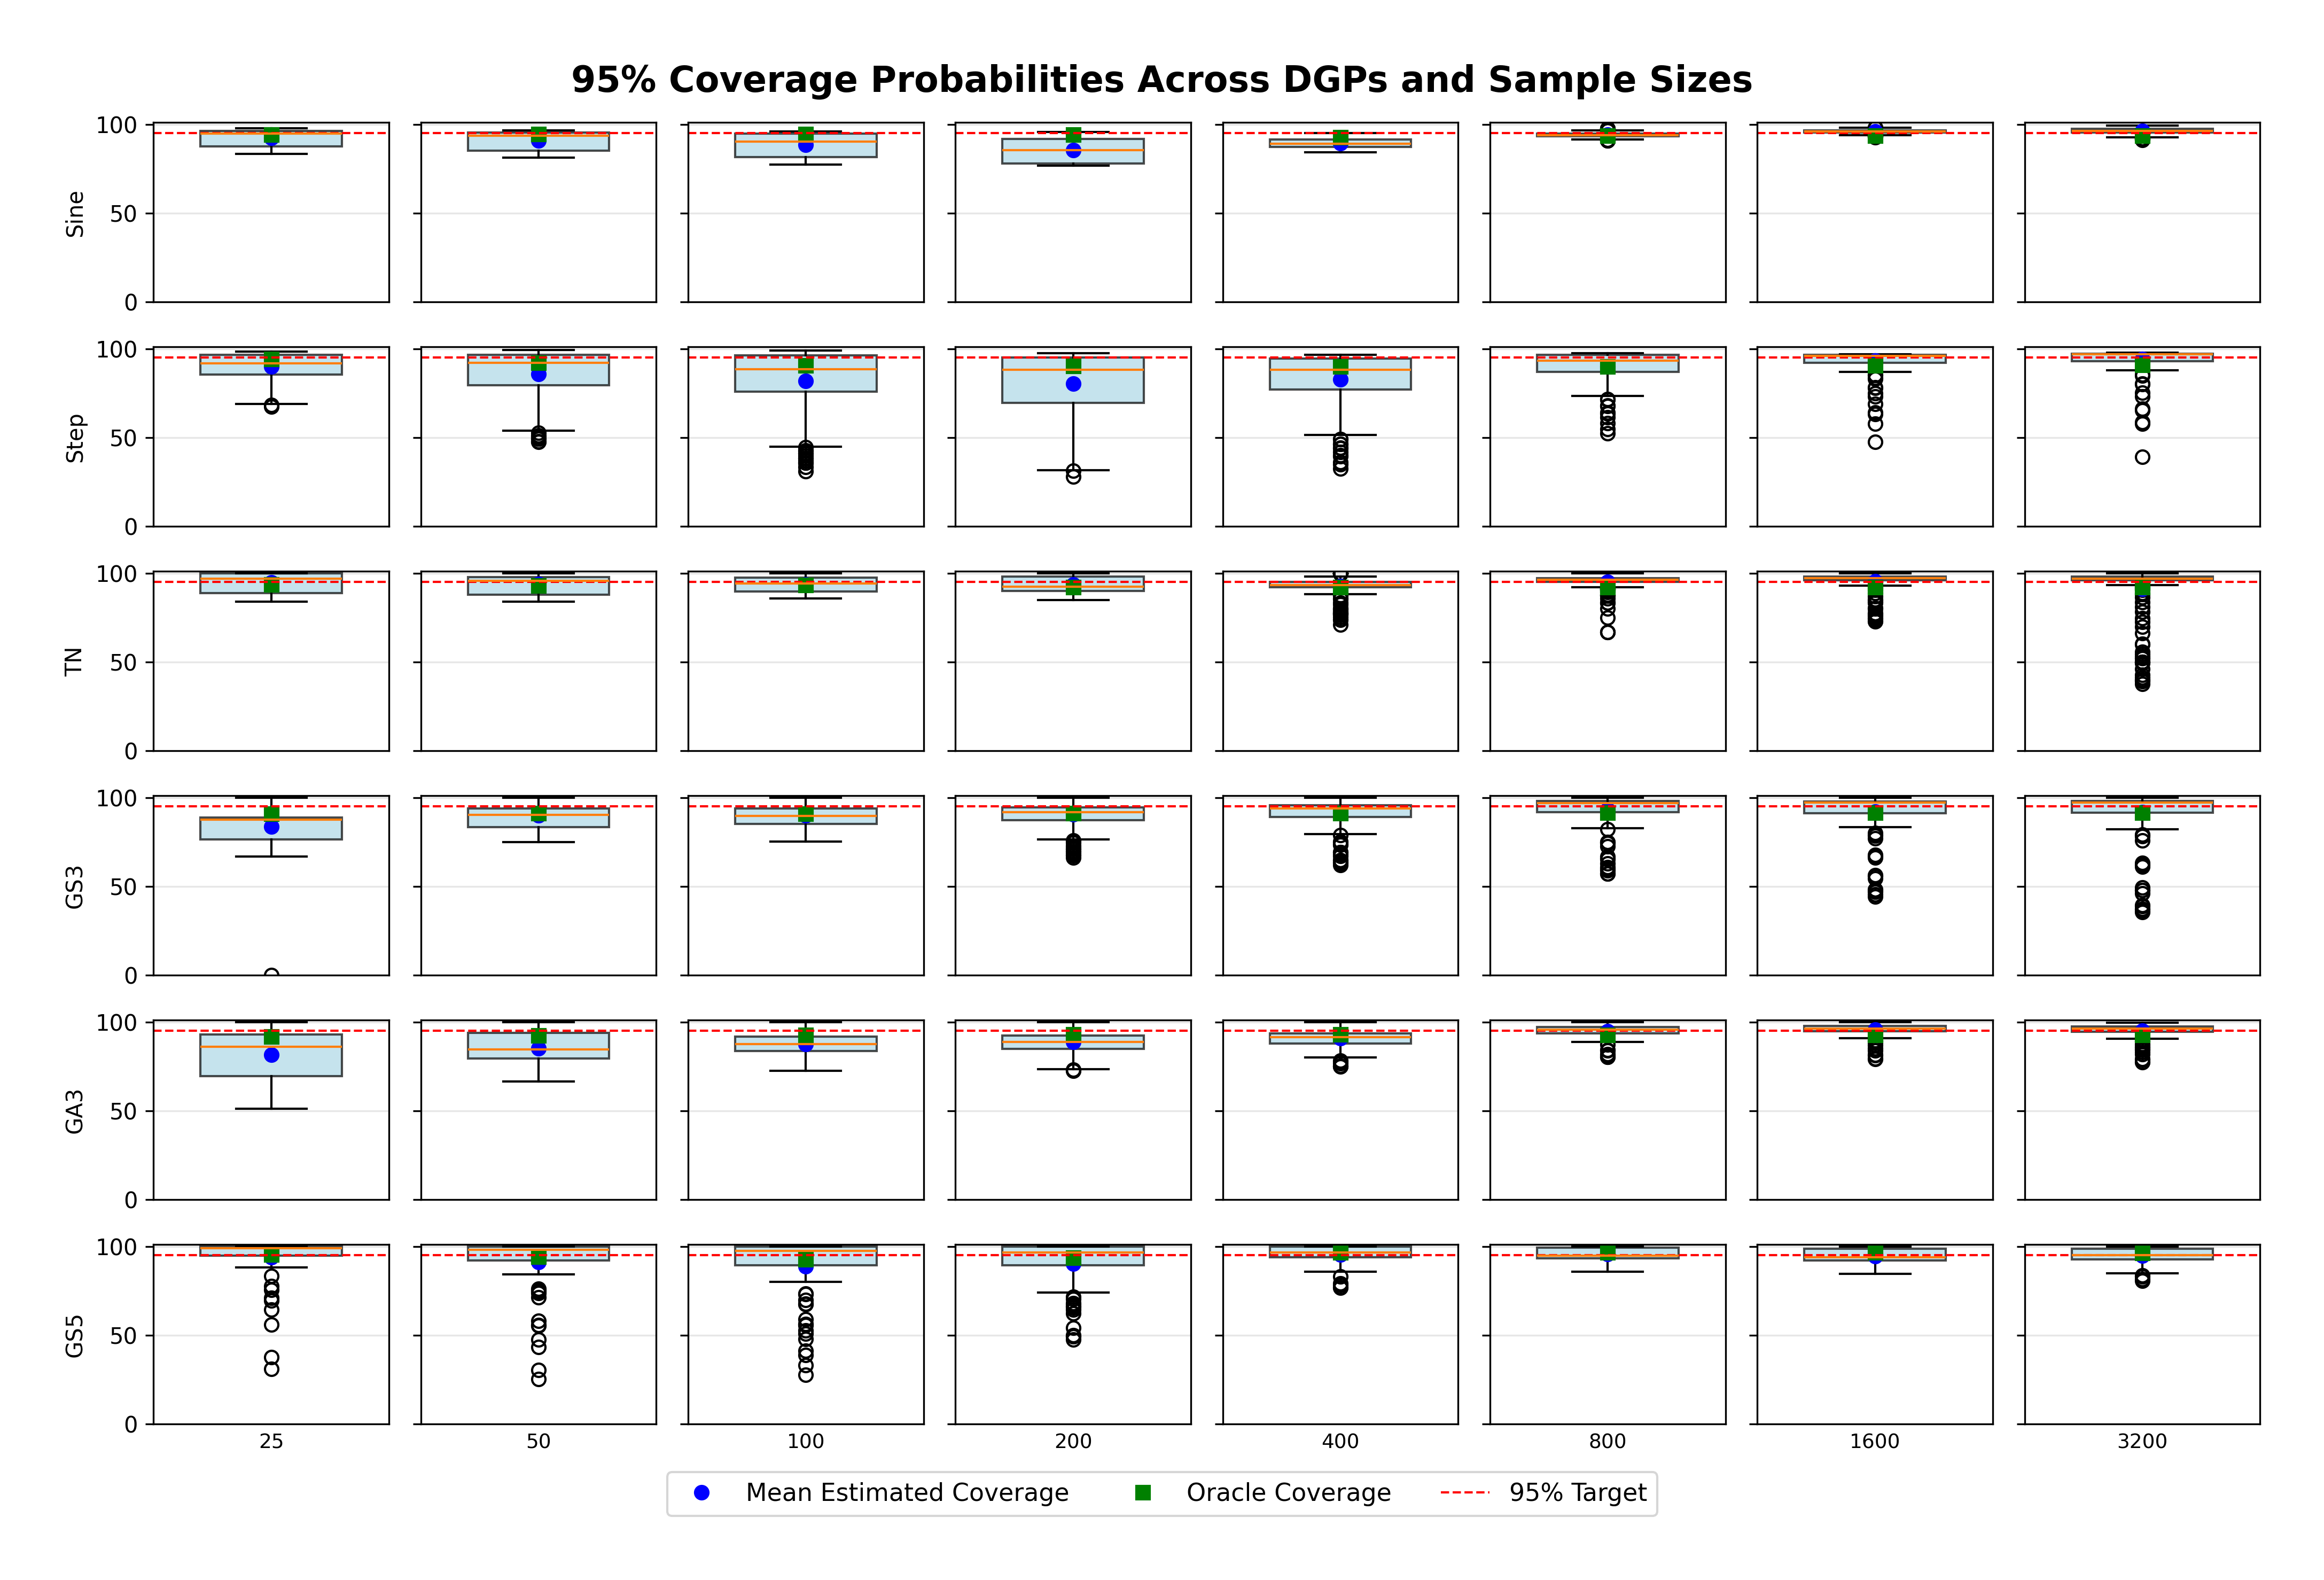
\includegraphics[angle=90, height=0.90\textheight]{resources/density_asymptotic_normality_and_var_est/Figure_Coverage_Combined.png}
    \caption{95\% coverage probabilities across DGPs and sample sizes (rotated for full\textendash page display).}
\end{figure}

\begin{figure}[p]
    \centering
    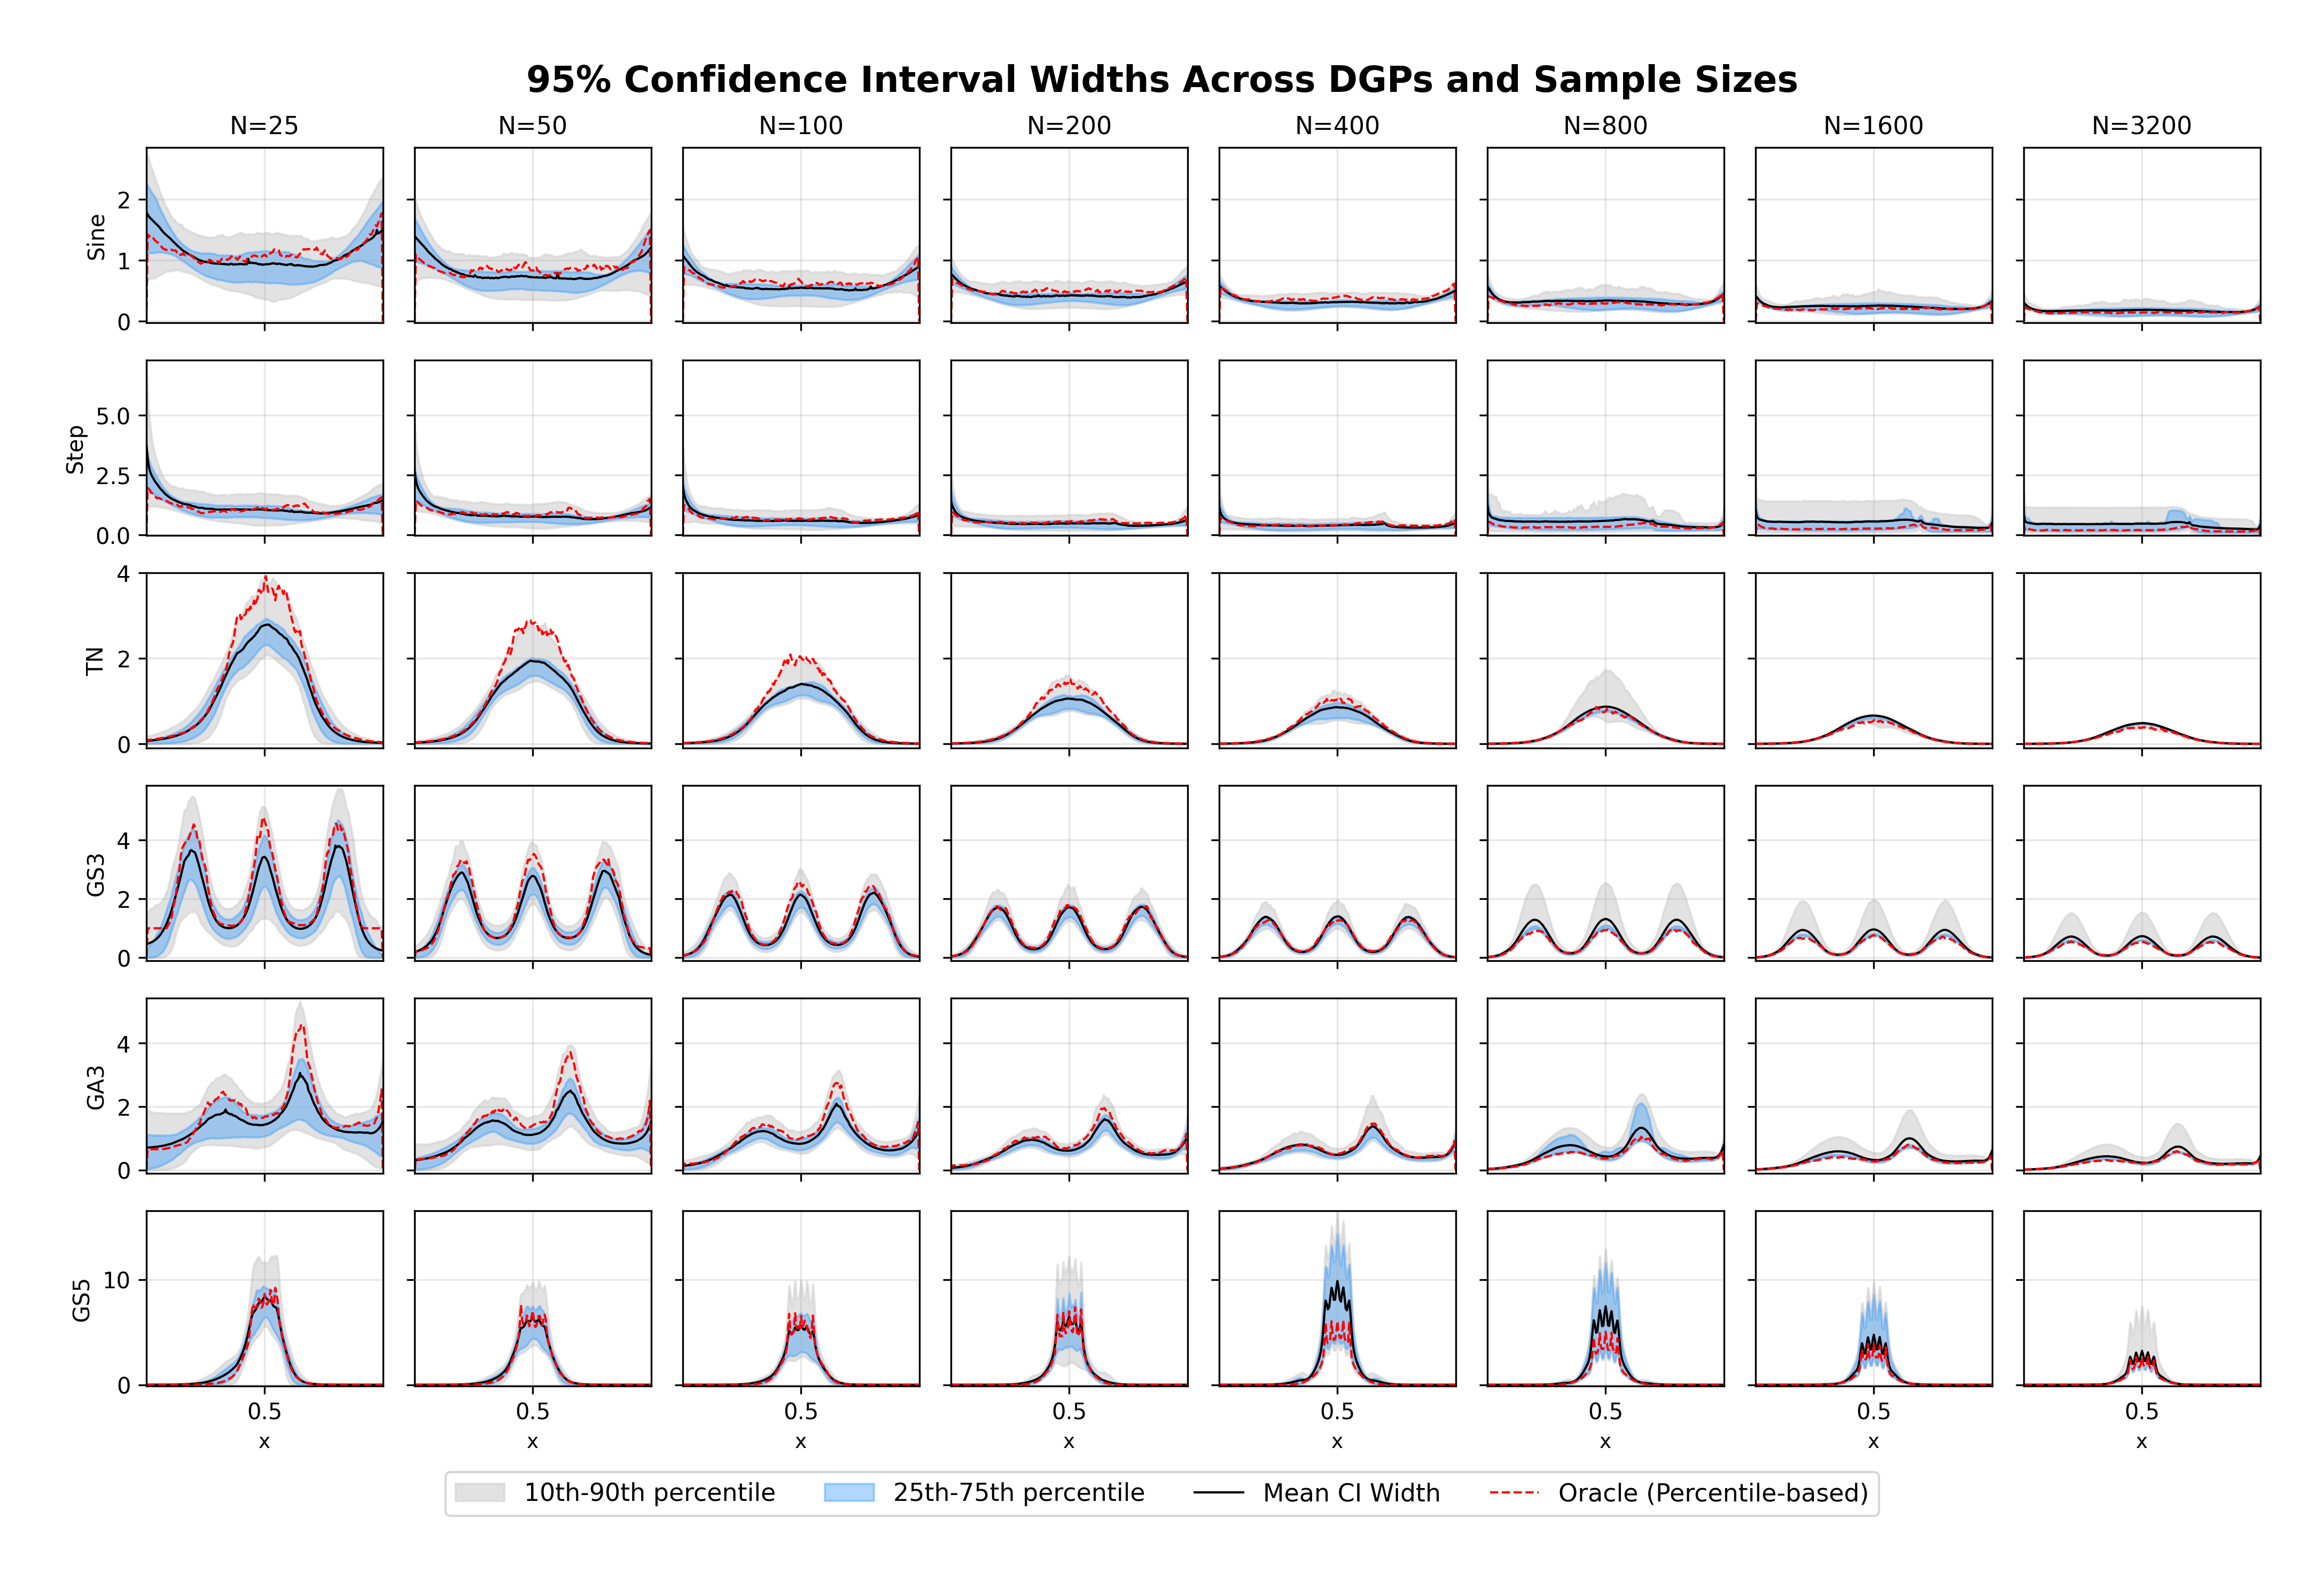
\includegraphics[angle=90, height=0.90\textheight]{resources/density_asymptotic_normality_and_var_est/Figure_CI_Widths_Combined.png}
    \caption{95\% confidence\textendash interval widths across DGPs and sample sizes (rotated for full\textendash page display).}
\end{figure}
\clearpage

\subsection{Asymptotic efficiency}\label{app_i_subsec:asymptotic_efficiency}
\begin{figure}[H]
    \centering
    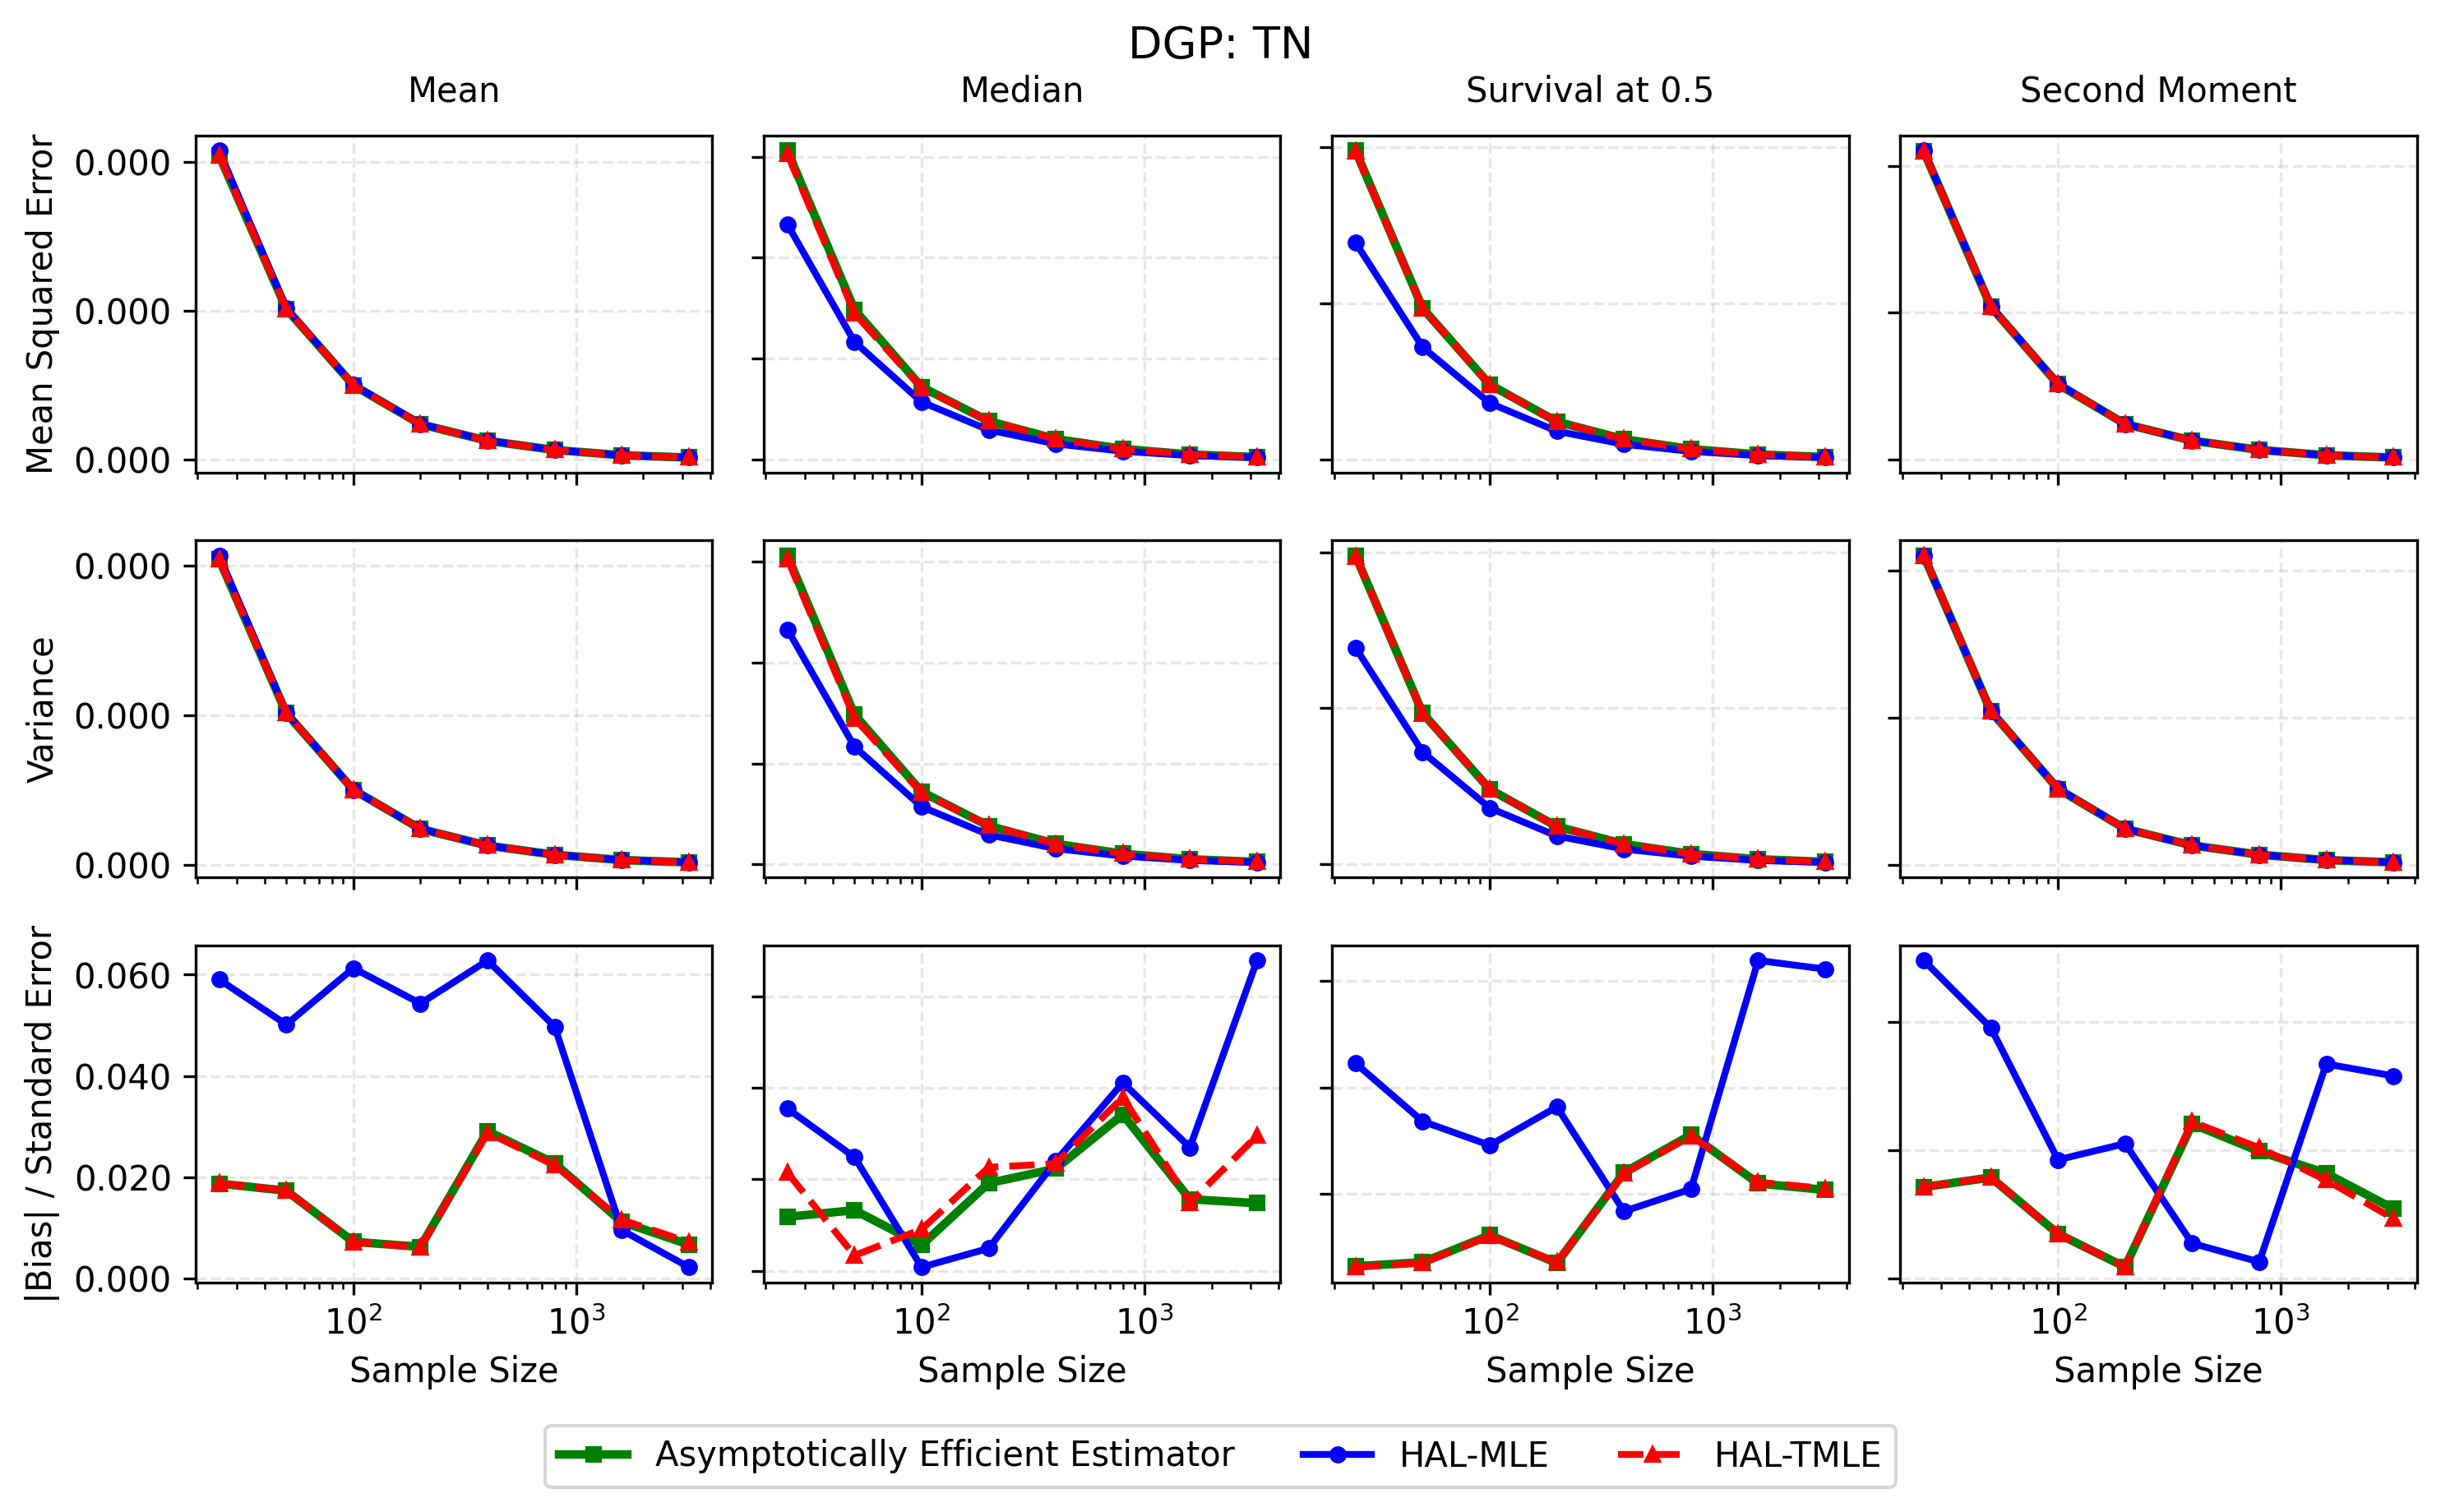
\includegraphics[width=0.9\textwidth]{resources/density_asymptotic_efficiency/TruncatedNormal/efficiency_comparison.png}
    \caption{Asymptotic\textendash efficiency comparison for TN.}
\end{figure}

\begin{figure}[H]
    \centering
    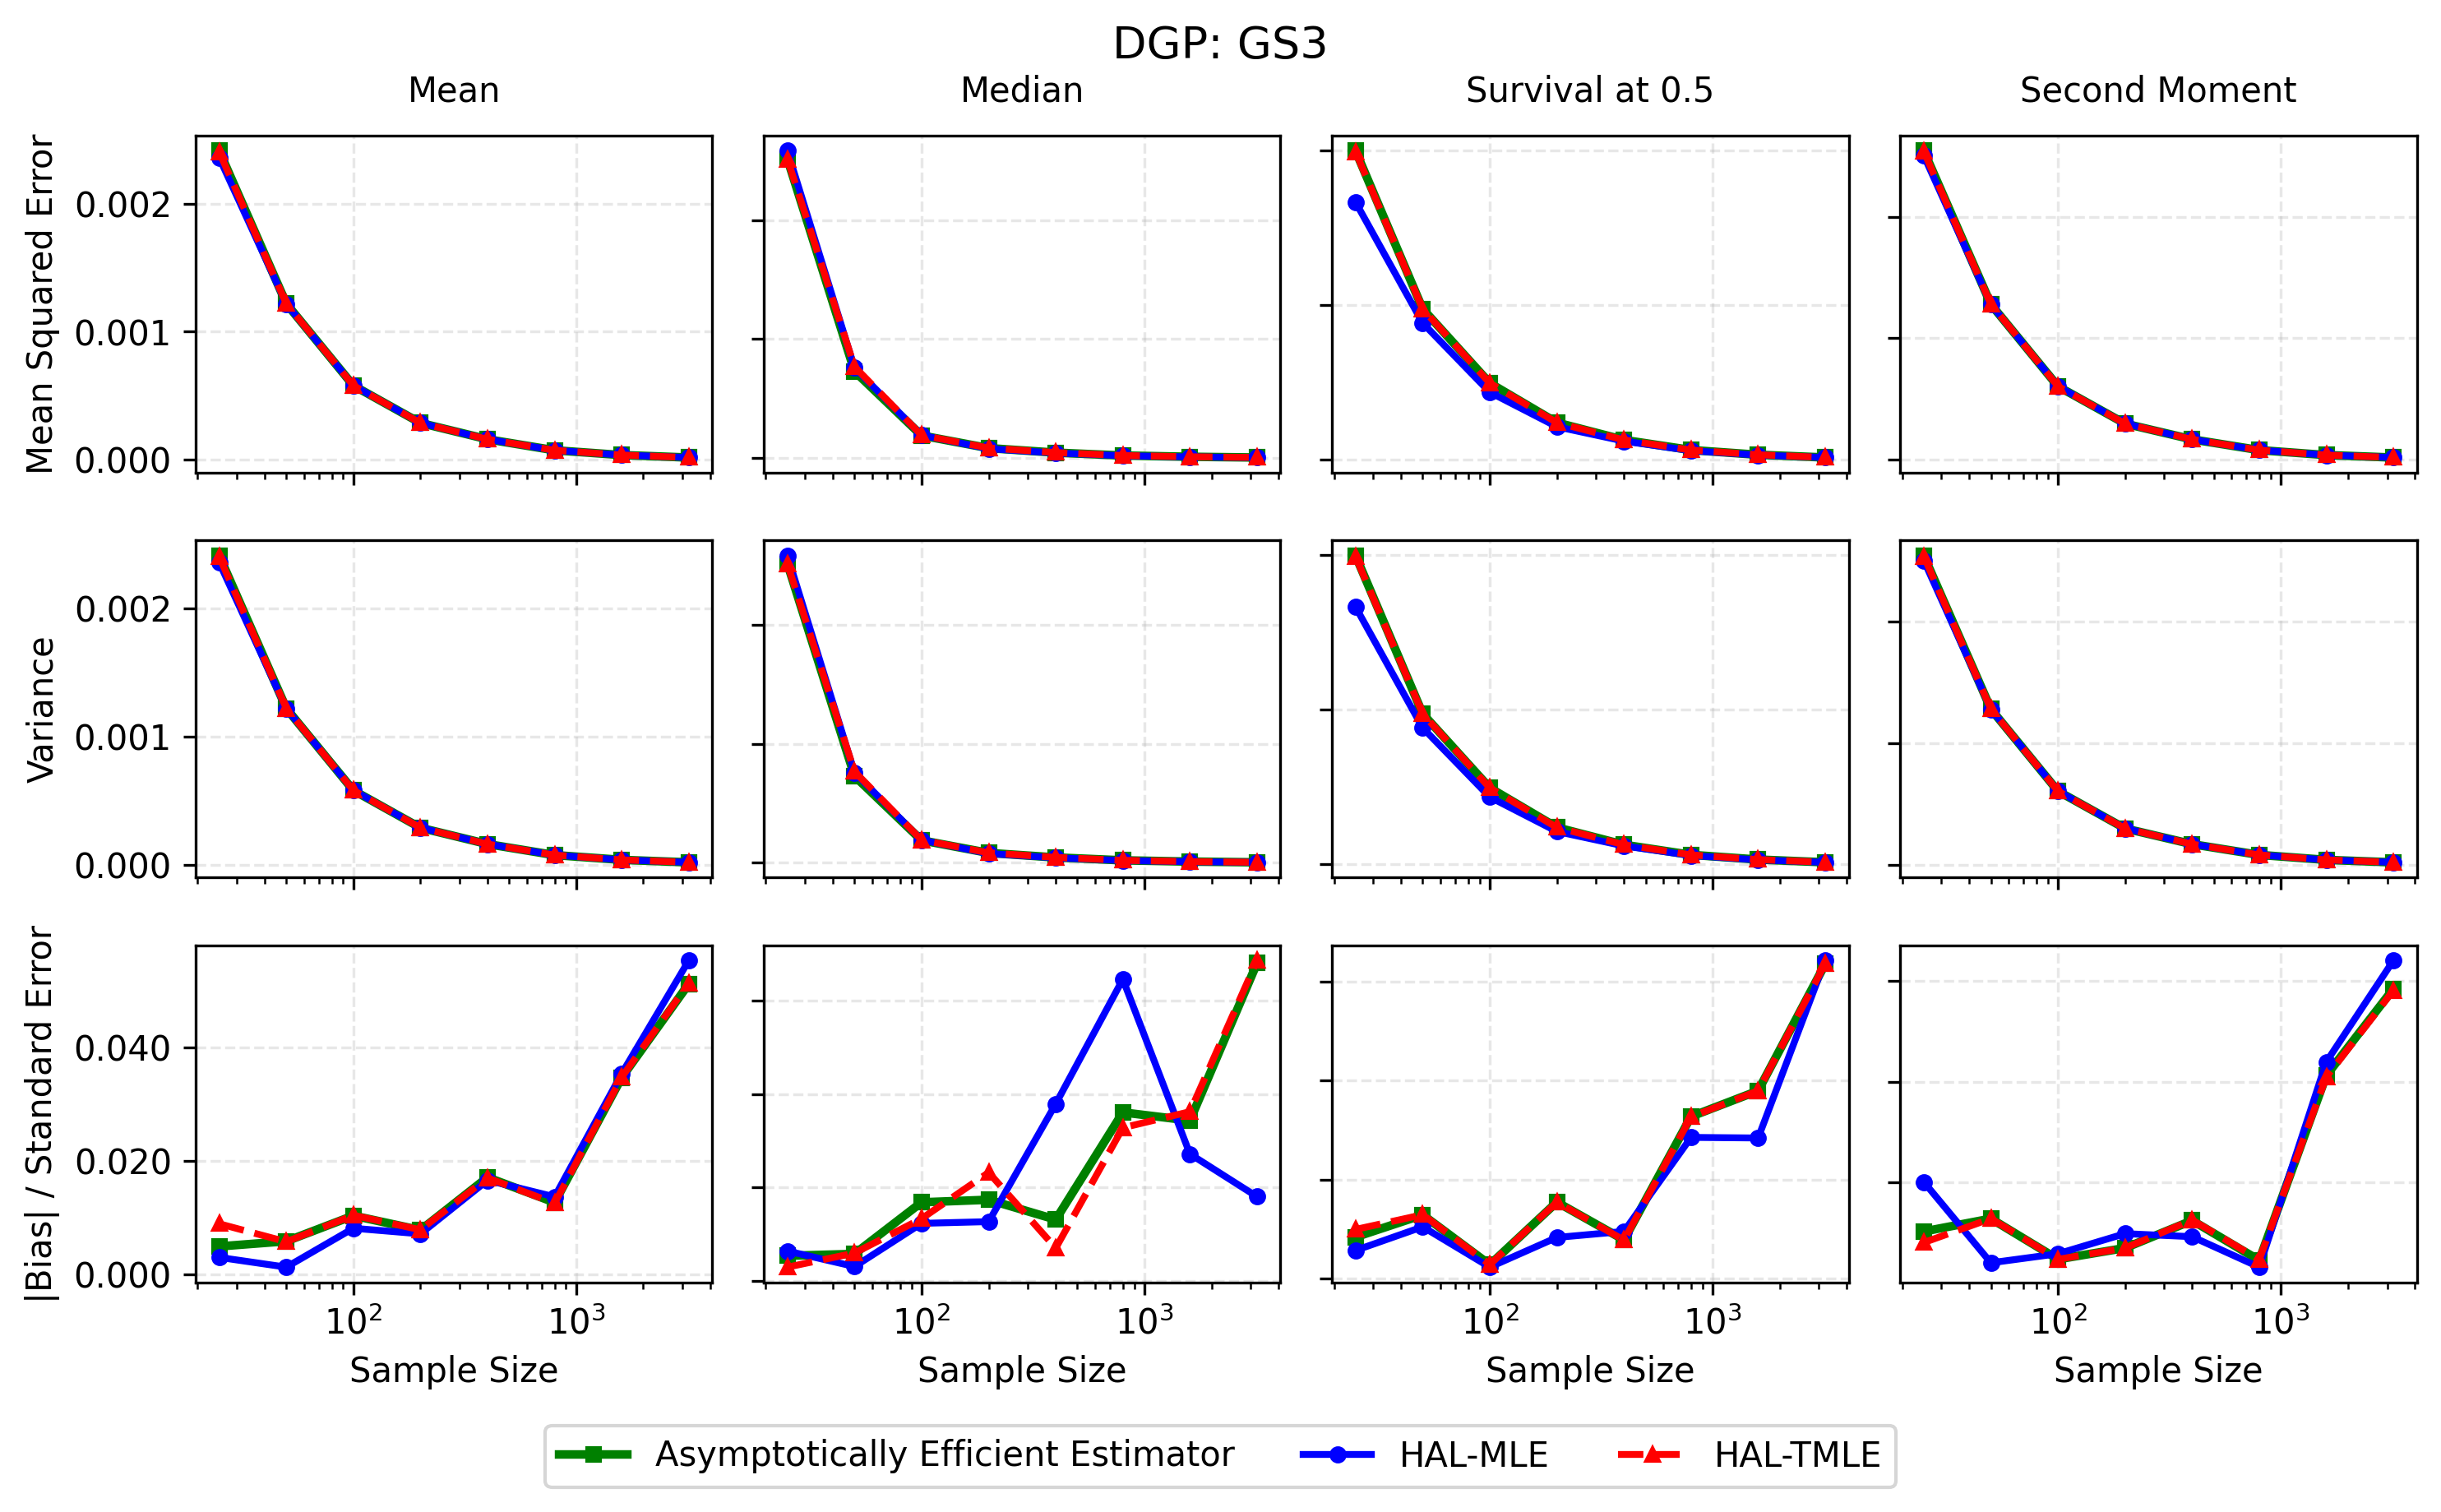
\includegraphics[width=0.9\textwidth]{resources/density_asymptotic_efficiency/TruncatedGMMSymmetricThree/efficiency_comparison.png}
    \caption{Asymptotic\textendash efficiency comparison for GS3.}
\end{figure}

\begin{figure}[H]
    \centering
    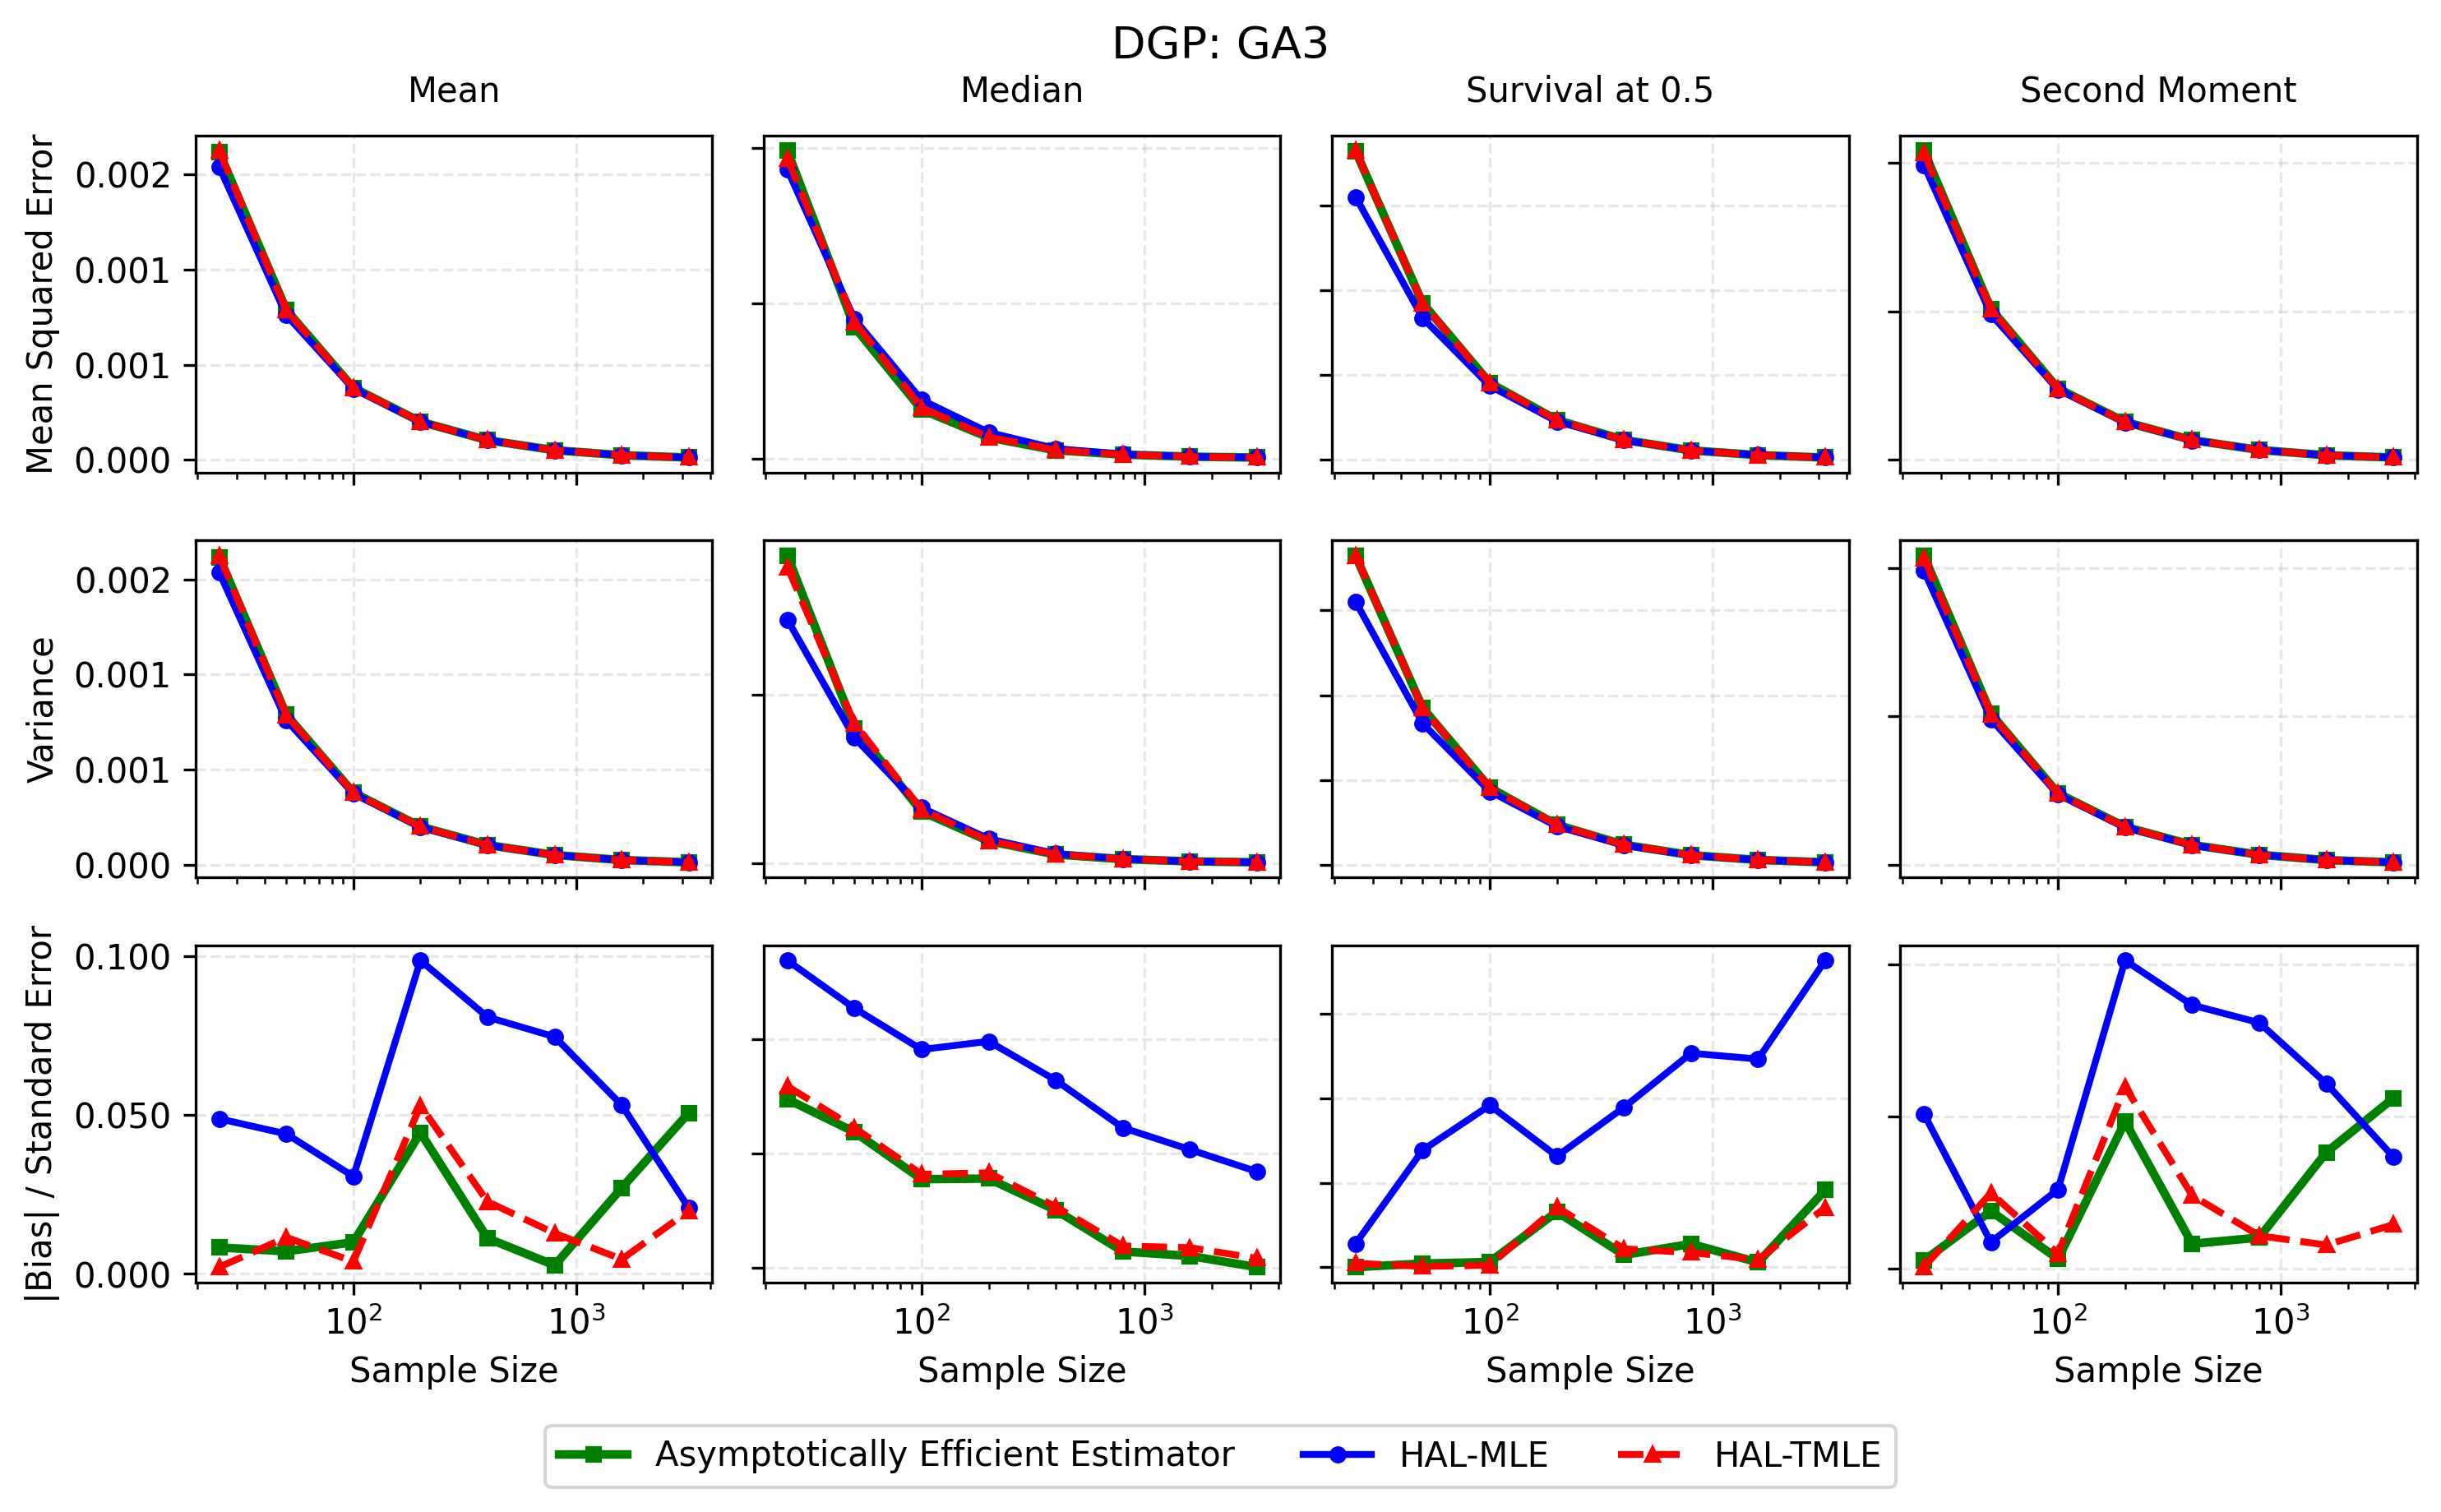
\includegraphics[width=0.9\textwidth]{resources/density_asymptotic_efficiency/TruncatedGMMAsymmetricThree/efficiency_comparison.png}
    \caption{Asymptotic\textendash efficiency comparison for GA3.}
\end{figure}

\begin{figure}[H]
    \centering
    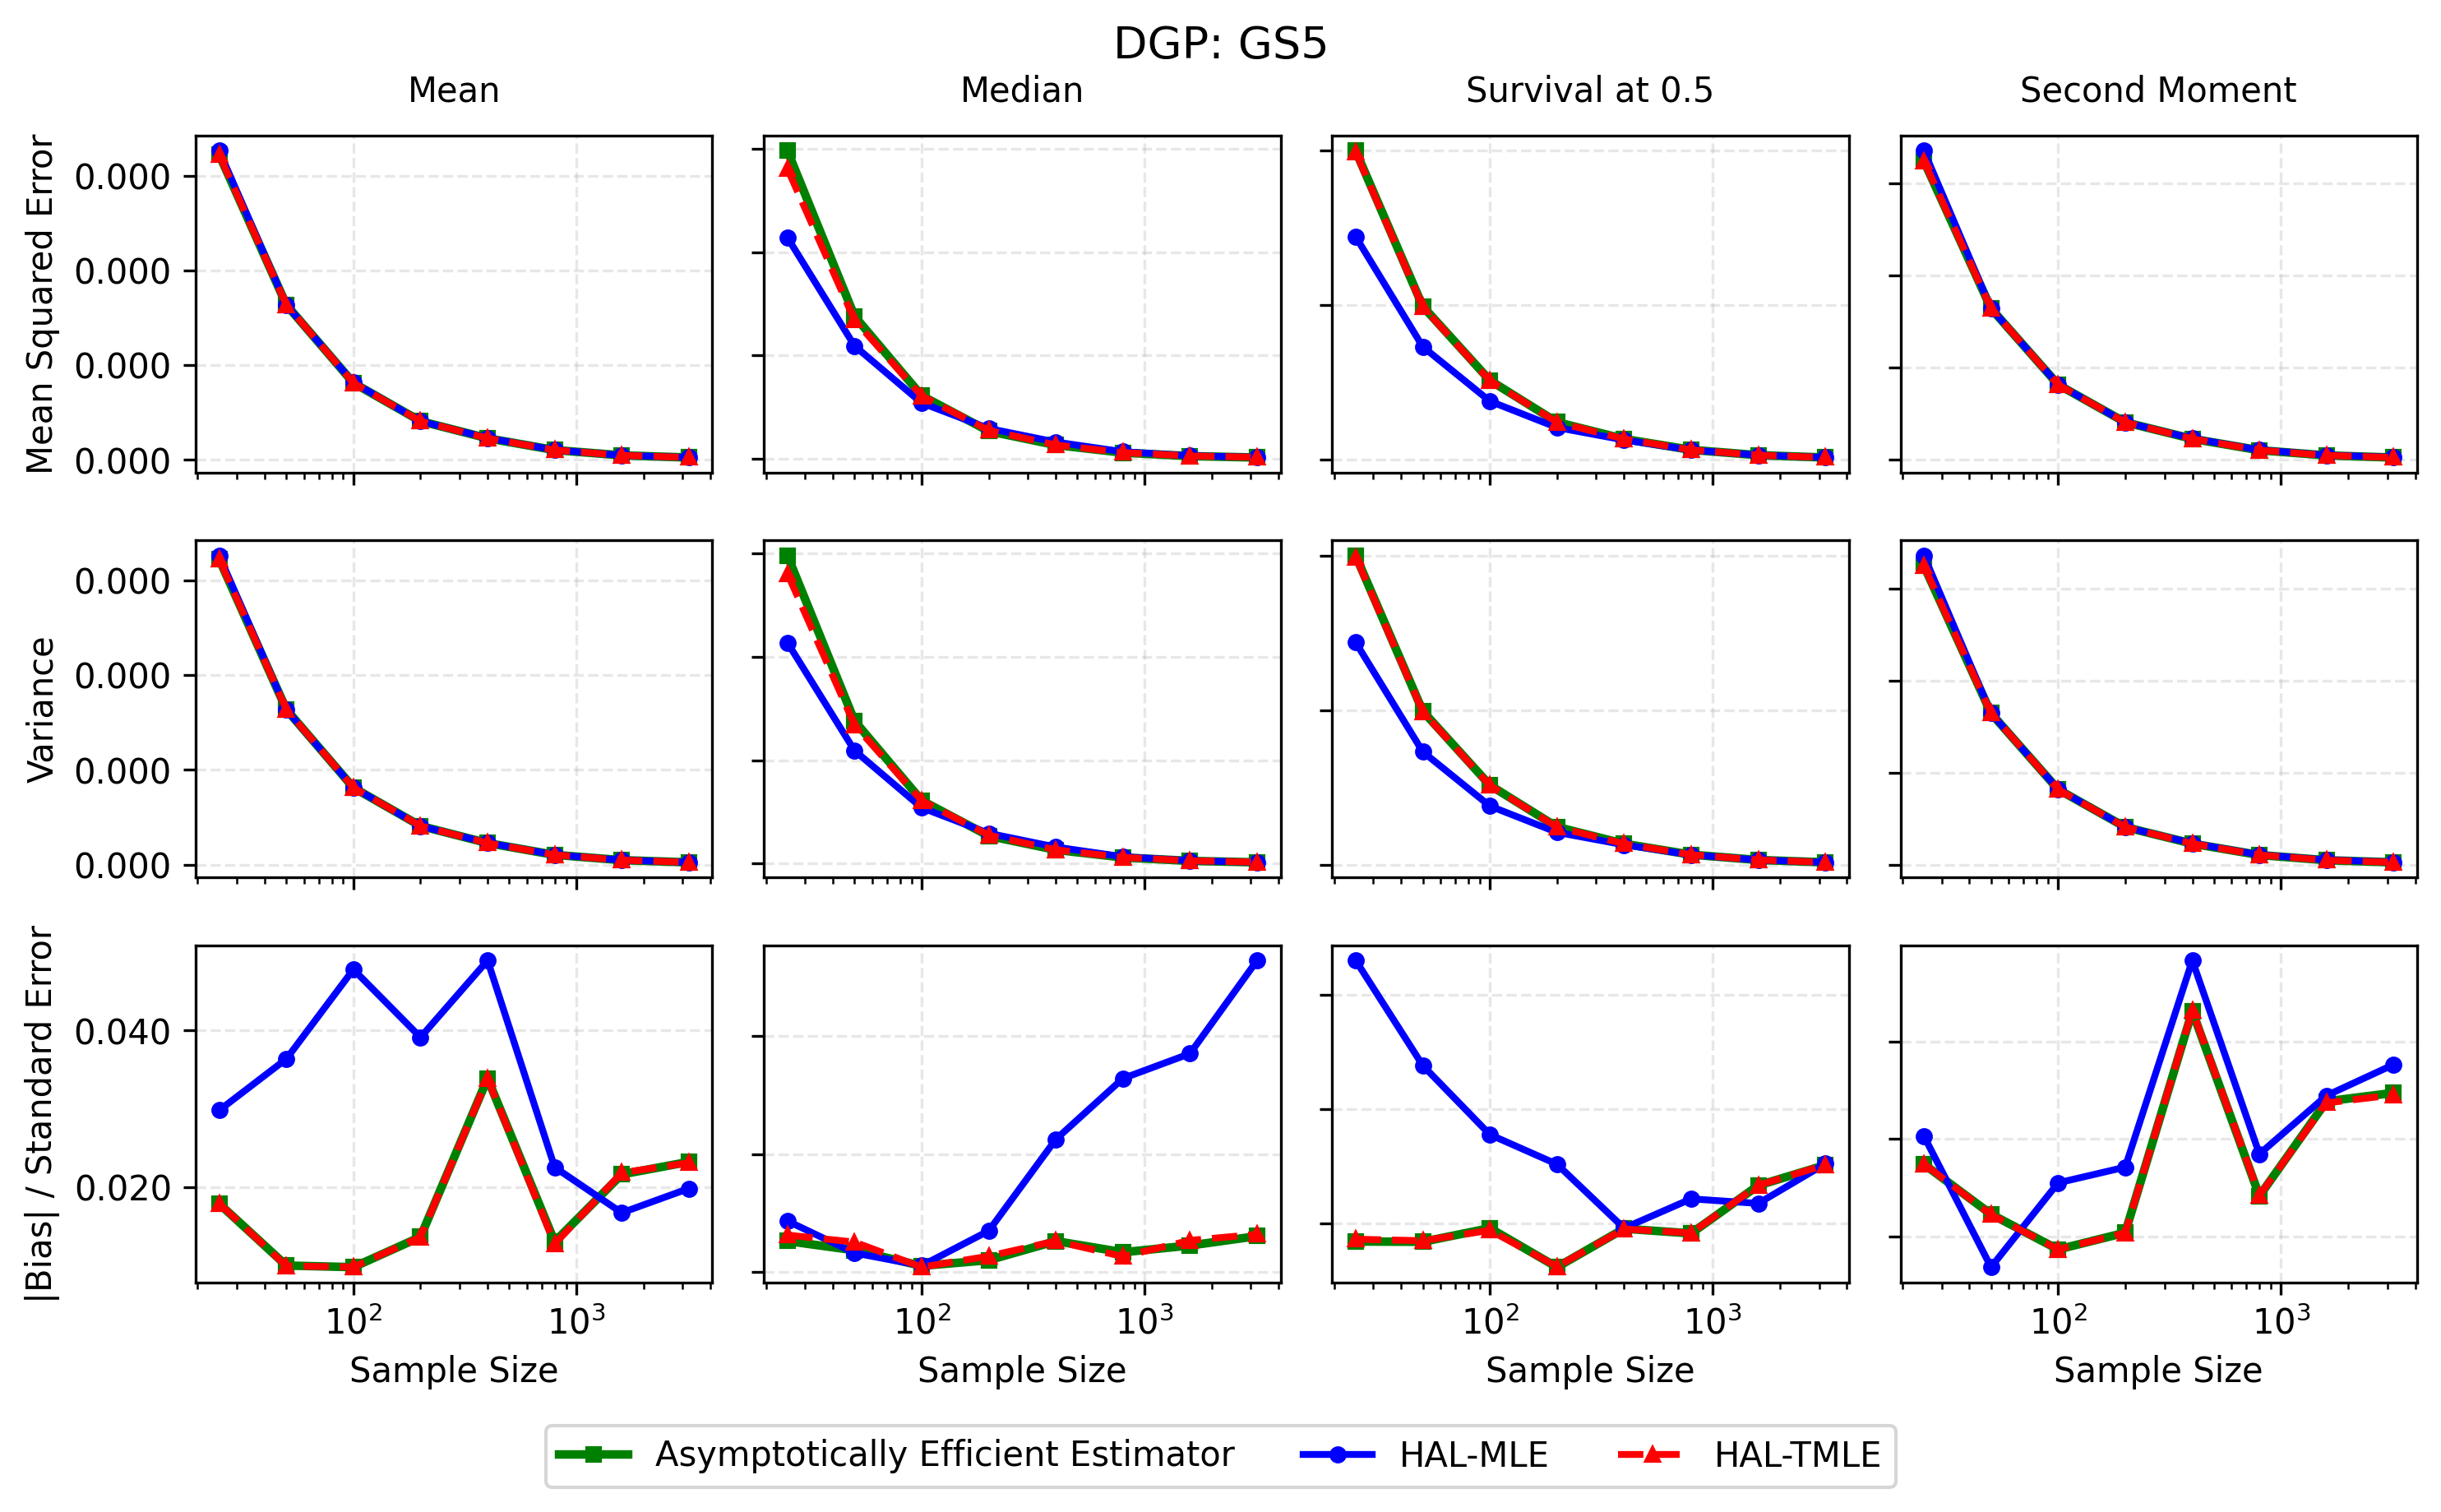
\includegraphics[width=0.9\textwidth]{resources/density_asymptotic_efficiency/TruncatedGMMFiveSpikes/efficiency_comparison.png}
    \caption{Asymptotic\textendash efficiency comparison for GS5.}
\end{figure}

\begin{figure}[H]
    \centering
    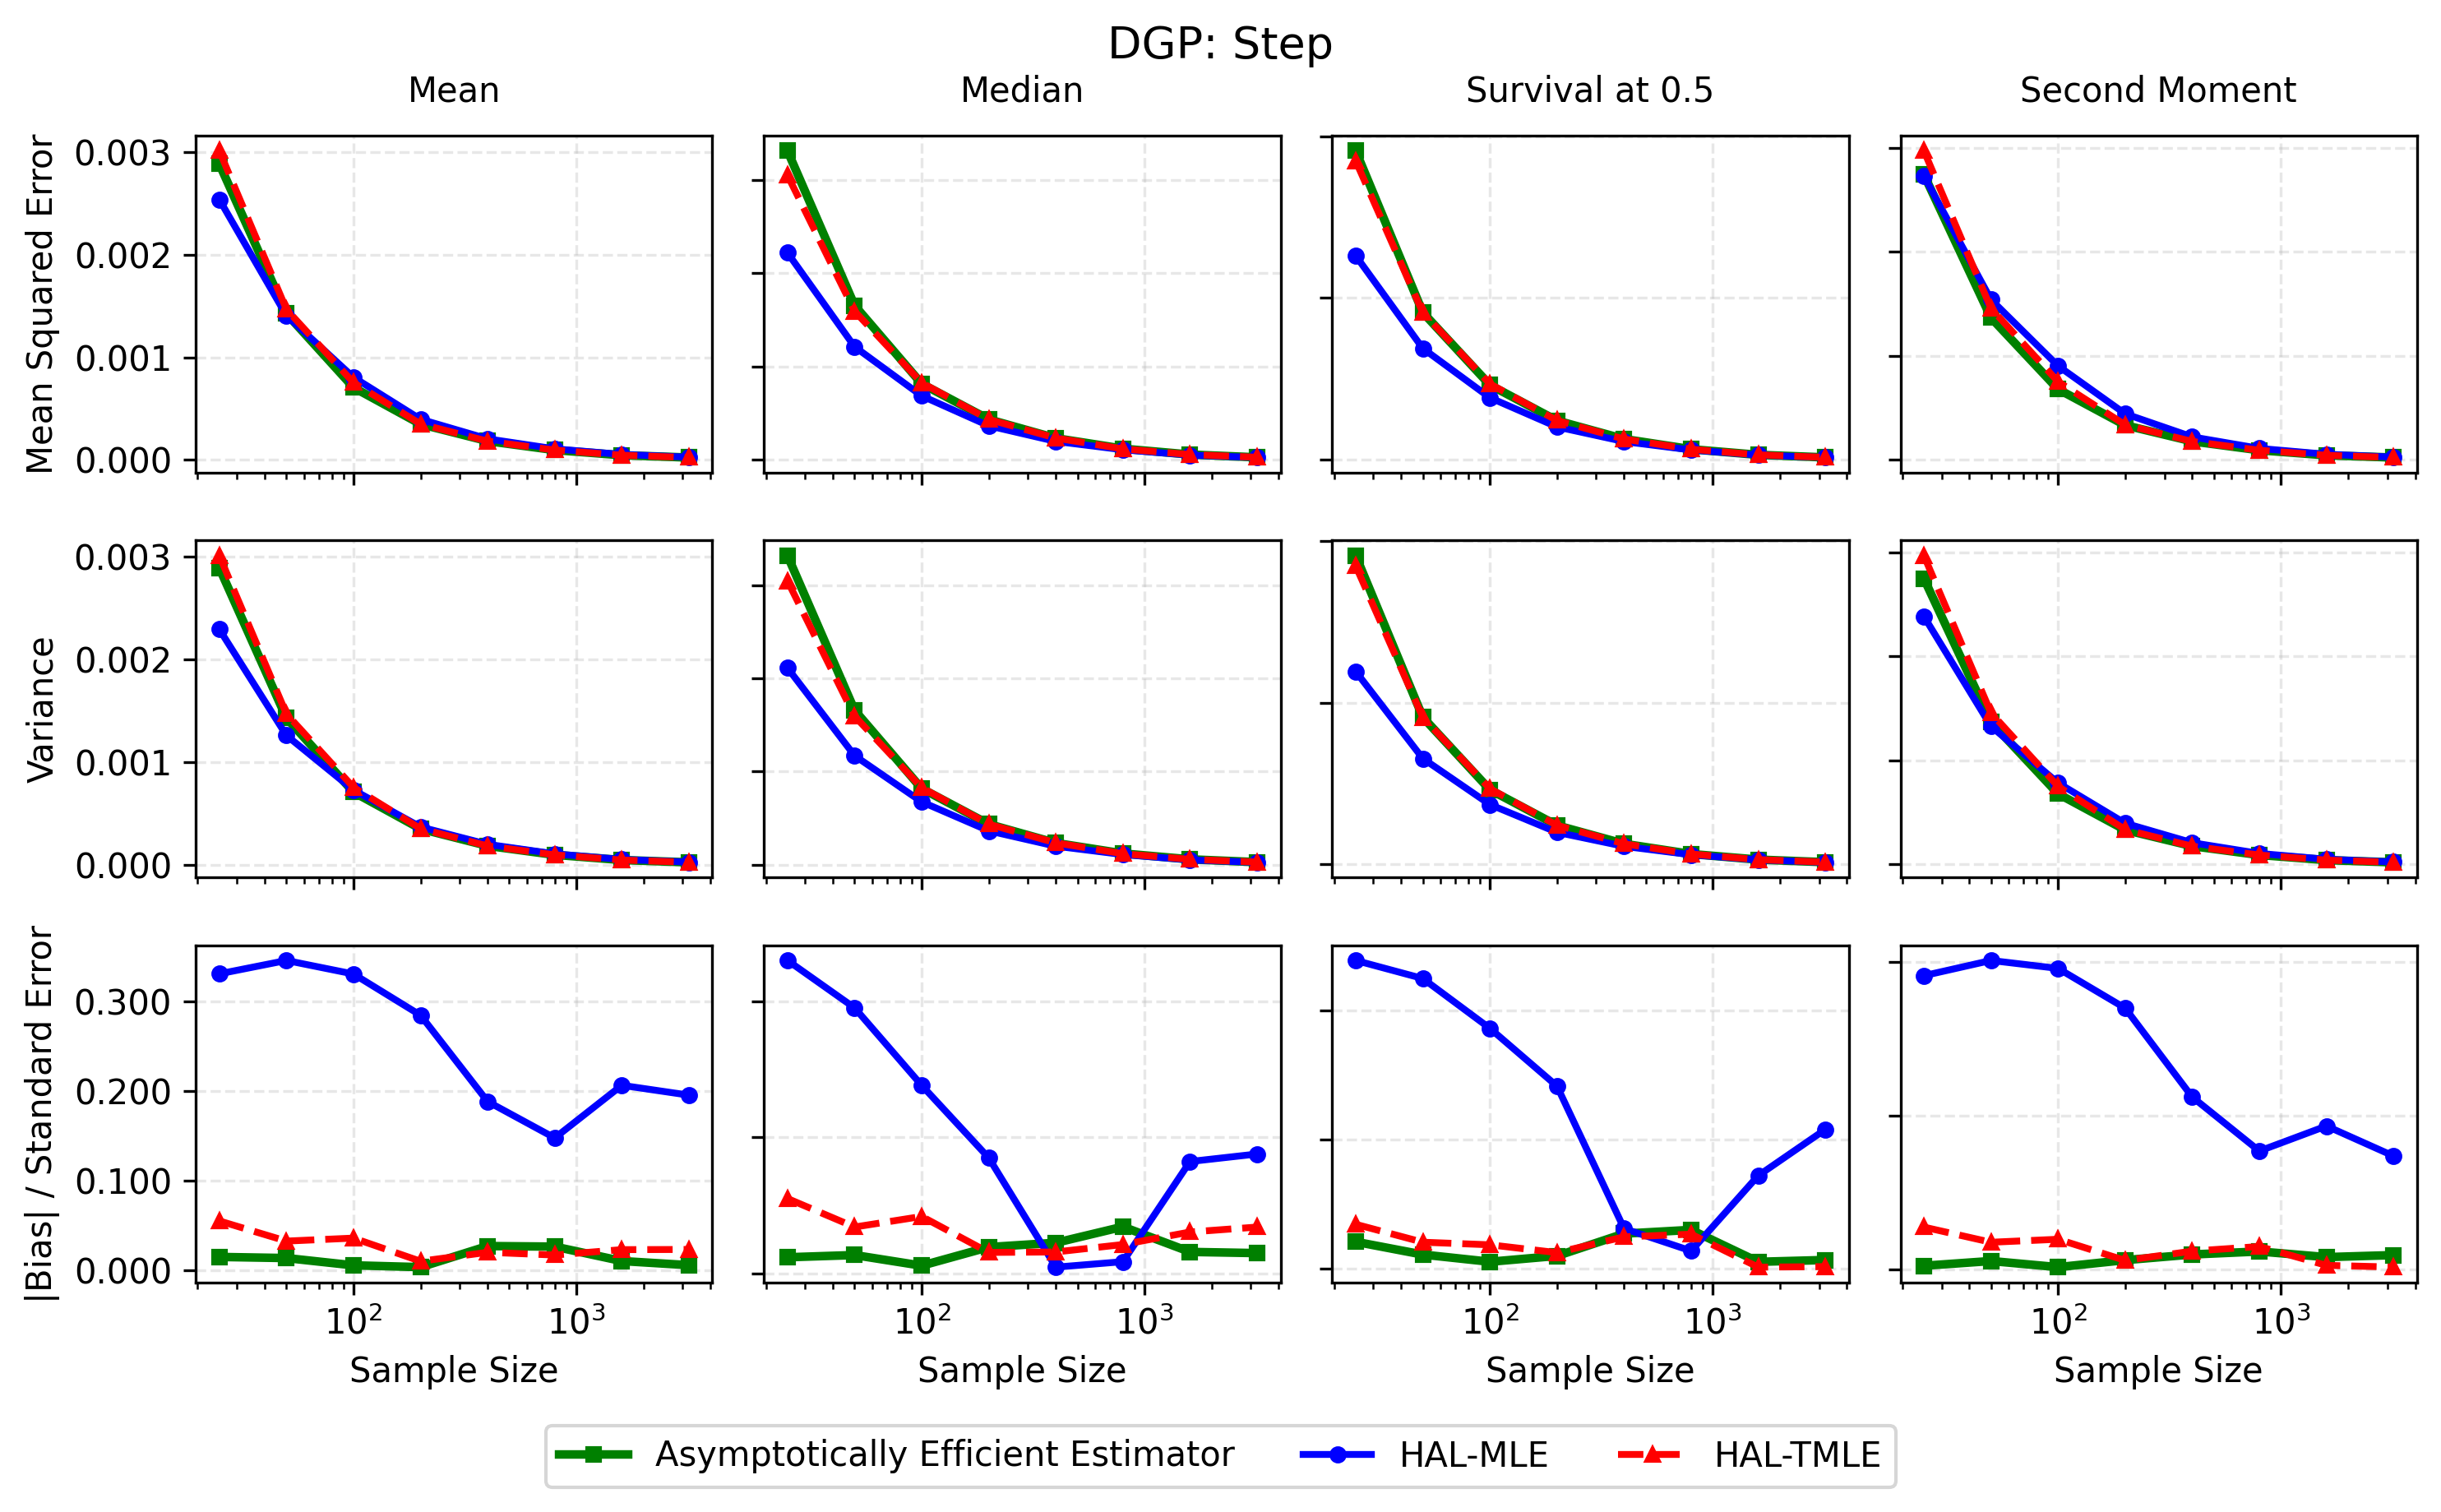
\includegraphics[width=0.9\textwidth]{resources/density_asymptotic_efficiency/StepFunction/efficiency_comparison.png}
    \caption{Asymptotic\textendash efficiency comparison for Step.}
\end{figure}

\begin{figure}[H]
    \centering
    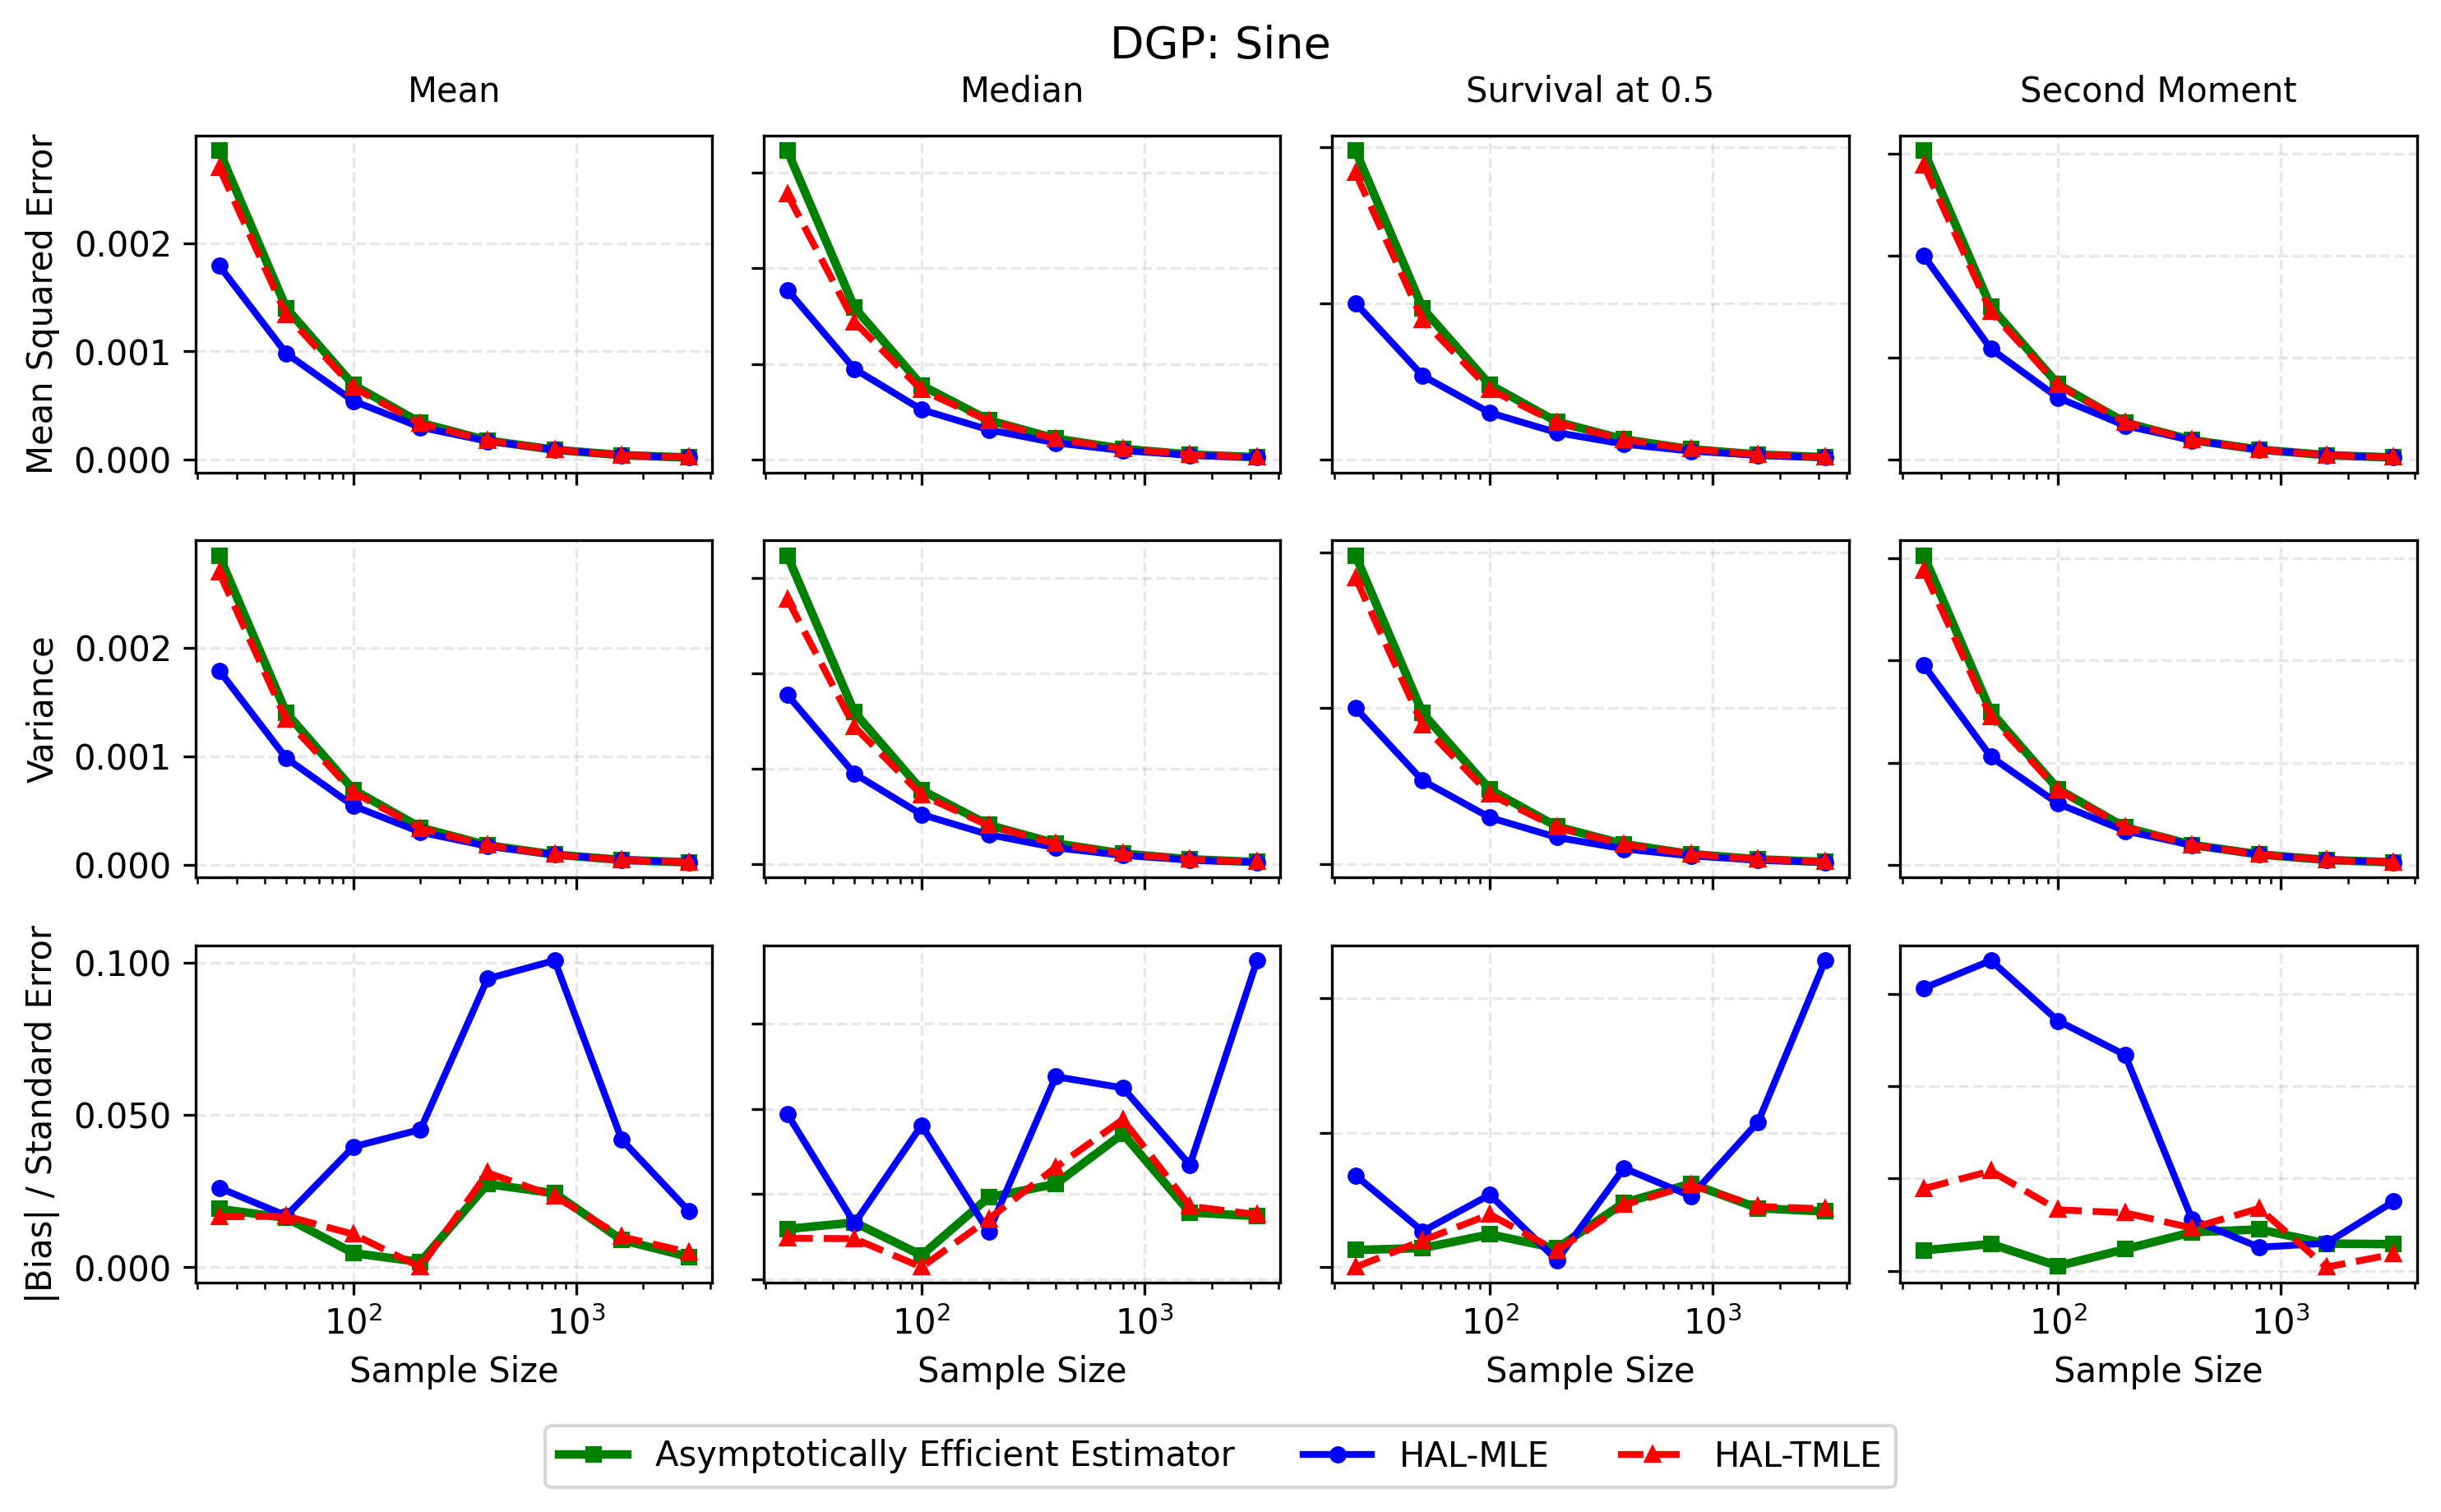
\includegraphics[width=0.9\textwidth]{resources/density_asymptotic_efficiency/Sinusoidal/efficiency_comparison.png}
    \caption{Asymptotic\textendash efficiency comparison for Sine.}
\end{figure}

\clearpage
\subsection{EIC\textendash based variance estimation for statistical estimands}\label{app_i_subsec:eic-based-variance-estimation}

% Auto-generated targeting coverage analysis table
\begin{table}[H]
  \centering
  \scriptsize
  \setlength{\tabcolsep}{2pt}
  \renewcommand{\arraystretch}{1.1}
  \begin{tabular}{lcccccccc}
    \toprule
    DGP & N=25 & N=50 & N=100 & N=200 & N=400 & N=800 & N=1600 & N=3200 \\
    \midrule
    TN & (93.3, 94.6) & (94.4, 96.0) & (94.9, 95.2) & (95.8, 95.4) & (94.7, 94.7) & (93.9, 95.1) & (95.3, 95.2) & (94.3, 94.3) \\
    GS3 & (95.1, 95.9) & (95.2, 95.8) & (95.7, 95.9) & (95.5, 94.9) & (94.3, 95.1) & (95.3, 94.9) & (95.1, 94.6) & (96.3, 96.1) \\
    GA3 & (94.8, 95.4) & (94.7, 95.3) & (95.6, 94.6) & (95.3, 95.0) & (94.9, 95.2) & (94.3, 94.2) & (96.2, 94.9) & (94.8, 94.6) \\
    GS5 & (95.5, 96.0) & (94.3, 94.7) & (96.2, 96.0) & (94.7, 94.5) & (93.1, 93.6) & (94.9, 94.8) & (95.5, 94.4) & (94.6, 94.0) \\
    Step & (93.5, 95.1) & (95.6, 96.4) & (92.6, 93.7) & (95.6, 95.3) & (94.0, 94.6) & (94.0, 95.1) & (95.2, 95.0) & (94.4, 94.3) \\
    Sine & (92.8, 93.6) & (95.1, 95.1) & (94.5, 94.7) & (95.8, 95.4) & (94.7, 94.9) & (94.3, 95.3) & (95.3, 95.3) & (94.4, 94.1) \\
    \bottomrule
  \end{tabular}
  \caption{Coverage for mean}
  \label{tab:coverage_targeting_mean}
\end{table}
% Auto-generated targeting coverage analysis table
\begin{table}[H]
  \centering
  \scriptsize
  \setlength{\tabcolsep}{2pt}
  \renewcommand{\arraystretch}{1.1}
  \begin{tabular}{lcccccccc}
    \toprule
    DGP & N=25 & N=50 & N=100 & N=200 & N=400 & N=800 & N=1600 & N=3200 \\
    \midrule
    TN & (93.2, 94.7) & (94.8, 95.4) & (94.1, 94.8) & (95.6, 95.1) & (94.5, 94.9) & (93.9, 95.1) & (95.2, 95.2) & (94.5, 94.3) \\
    GS3 & (94.9, 95.3) & (94.9, 95.6) & (95.6, 95.7) & (95.4, 95.0) & (94.0, 94.4) & (94.6, 94.8) & (95.2, 94.7) & (96.7, 95.1) \\
    GA3 & (94.3, 95.6) & (94.4, 95.1) & (95.8, 95.1) & (95.0, 95.0) & (95.5, 95.8) & (93.9, 94.3) & (95.8, 95.1) & (95.6, 95.1) \\
    GS5 & (95.5, 96.0) & (94.2, 94.8) & (96.0, 96.1) & (95.3, 95.1) & (93.2, 94.1) & (94.8, 94.8) & (95.2, 94.4) & (94.9, 94.1) \\
    Step & (92.8, 96.0) & (94.8, 96.9) & (91.4, 94.4) & (94.9, 95.7) & (93.5, 94.0) & (94.0, 95.1) & (95.2, 95.1) & (94.2, 93.8) \\
    Sine & (93.3, 94.2) & (94.6, 95.0) & (94.1, 94.6) & (95.2, 95.4) & (93.4, 93.5) & (94.2, 95.1) & (94.7, 94.7) & (94.7, 94.0) \\
    \bottomrule
  \end{tabular}
  \caption{Coverage for second moment}
  \label{tab:coverage_targeting_second_moment}
\end{table}
% Auto-generated targeting coverage analysis table
\begin{table}[H]
  \centering
  \scriptsize
  \setlength{\tabcolsep}{2pt}
  \renewcommand{\arraystretch}{1.1}
  \begin{tabular}{lcccccccc}
    \toprule
    DGP & N=25 & N=50 & N=100 & N=200 & N=400 & N=800 & N=1600 & N=3200 \\
    \midrule
    TN & (95.4, 95.4) & (94.4, 94.4) & (95.0, 95.0) & (95.4, 95.4) & (94.4, 94.7) & (95.4, 95.5) & (95.5, 95.5) & (95.2, 94.6) \\
    GS3 & (95.9, 95.9) & (93.6, 93.6) & (94.8, 94.8) & (95.0, 95.0) & (94.5, 94.7) & (95.8, 95.5) & (93.8, 93.8) & (96.5, 94.5) \\
    GA3 & (94.2, 96.5) & (96.0, 95.3) & (93.2, 94.8) & (93.9, 94.9) & (95.3, 95.3) & (95.6, 95.0) & (96.1, 95.4) & (95.8, 95.5) \\
    GS5 & (96.1, 96.1) & (93.1, 94.3) & (94.4, 95.1) & (95.9, 95.7) & (94.3, 95.1) & (94.8, 95.4) & (94.8, 94.7) & (95.1, 94.8) \\
    Step & (93.4, 96.2) & (95.1, 96.8) & (96.2, 95.8) & (94.8, 95.5) & (93.9, 94.6) & (94.3, 94.5) & (96.0, 96.0) & (95.0, 94.2) \\
    Sine & (95.4, 95.4) & (94.5, 94.5) & (95.1, 95.1) & (95.4, 95.4) & (94.4, 94.4) & (94.9, 95.6) & (95.3, 95.4) & (95.2, 94.6) \\
    \bottomrule
  \end{tabular}
  \caption{Coverage for survival at 0.5}
  \label{tab:coverage_targeting_survival_0_5}
\end{table}
% Auto-generated targeting coverage analysis table
\begin{table}[H]
  \centering
  \scriptsize
  \setlength{\tabcolsep}{2pt}
  \renewcommand{\arraystretch}{1.1}
  \begin{tabular}{lcccccccc}
    \toprule
    DGP & N=25 & N=50 & N=100 & N=200 & N=400 & N=800 & N=1600 & N=3200 \\
    \midrule
    TN & (91.5, 94.3) & (94.0, 94.8) & (95.5, 95.9) & (95.0, 94.9) & (94.7, 95.5) & (94.8, 95.5) & (95.4, 95.6) & (95.4, 94.5) \\
    GS3 & (93.8, 92.8) & (97.0, 95.8) & (97.7, 94.7) & (96.6, 95.3) & (94.7, 94.9) & (94.9, 95.2) & (93.6, 94.1) & (96.2, 95.1) \\
    GA3 & (89.8, 91.3) & (92.4, 93.8) & (93.7, 94.5) & (96.3, 94.7) & (96.7, 94.4) & (96.1, 94.8) & (96.7, 95.1) & (95.0, 94.8) \\
    GS5 & (91.2, 94.8) & (92.7, 93.4) & (95.6, 94.7) & (96.7, 94.9) & (96.5, 94.0) & (96.3, 95.9) & (95.2, 94.8) & (96.4, 94.6) \\
    Step & (91.8, 95.2) & (93.3, 95.5) & (94.7, 96.3) & (93.7, 94.6) & (94.2, 95.4) & (95.1, 95.6) & (95.8, 96.3) & (95.8, 95.2) \\
    Sine & (91.9, 94.0) & (93.7, 94.1) & (95.1, 94.5) & (94.2, 94.5) & (95.2, 95.2) & (94.7, 95.1) & (95.7, 96.0) & (96.1, 95.3) \\
    \bottomrule
  \end{tabular}
  \caption{Coverage for median}
  \label{tab:coverage_targeting_median}
\end{table}

\clearpage
\begin{figure}[H]
    \centering
    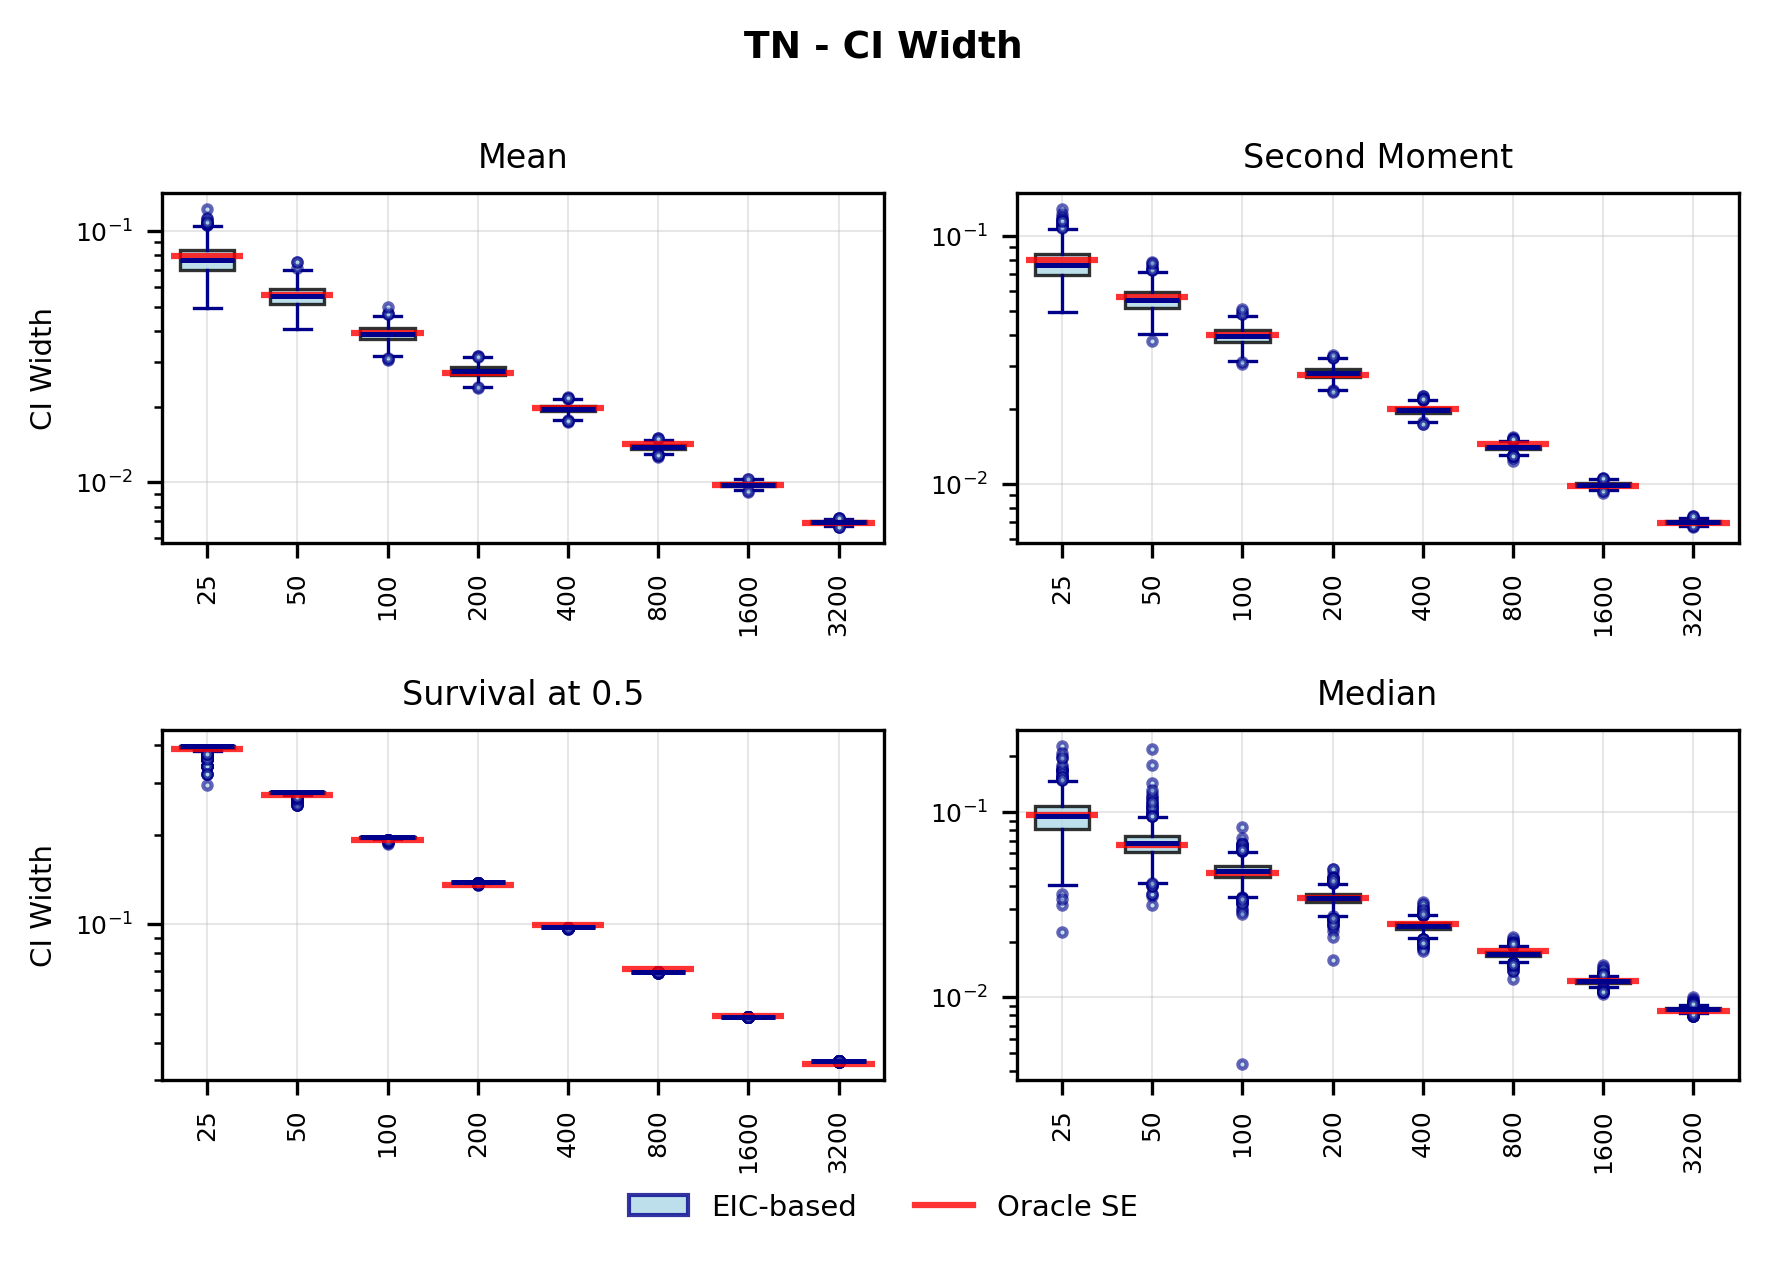
\includegraphics[width=0.75\textwidth]{resources/target_estimand_variance/Figure_CI_Width_TruncatedNormal.png}
    \caption{EIC\textendash based variance estimation for TN: CI width.}
\end{figure}

\begin{figure}[H]
    \centering
    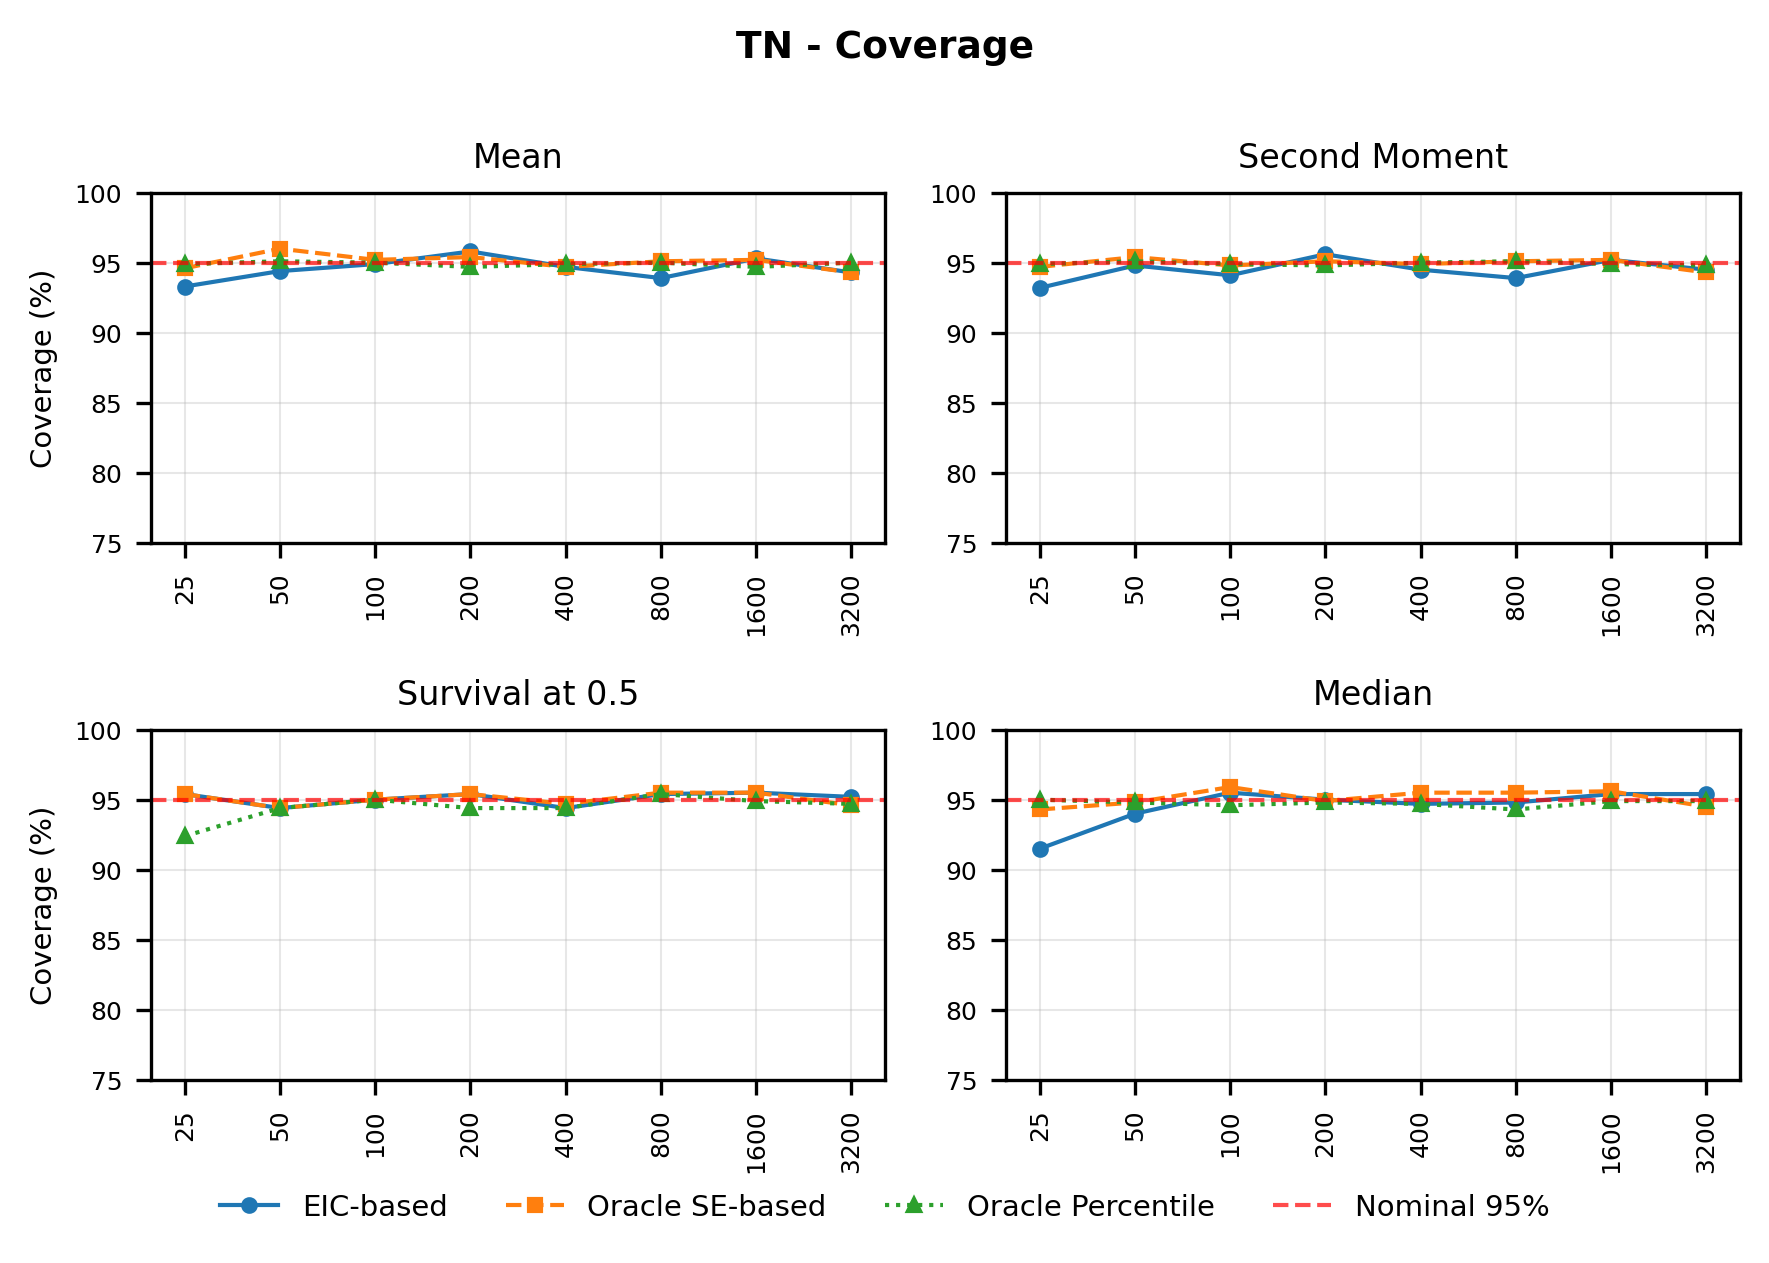
\includegraphics[width=0.75\textwidth]{resources/target_estimand_variance/Figure_Coverage_TruncatedNormal.png}
    \caption{EIC\textendash based variance estimation for TN: coverage.}
\end{figure}

\begin{figure}[H]
    \centering
    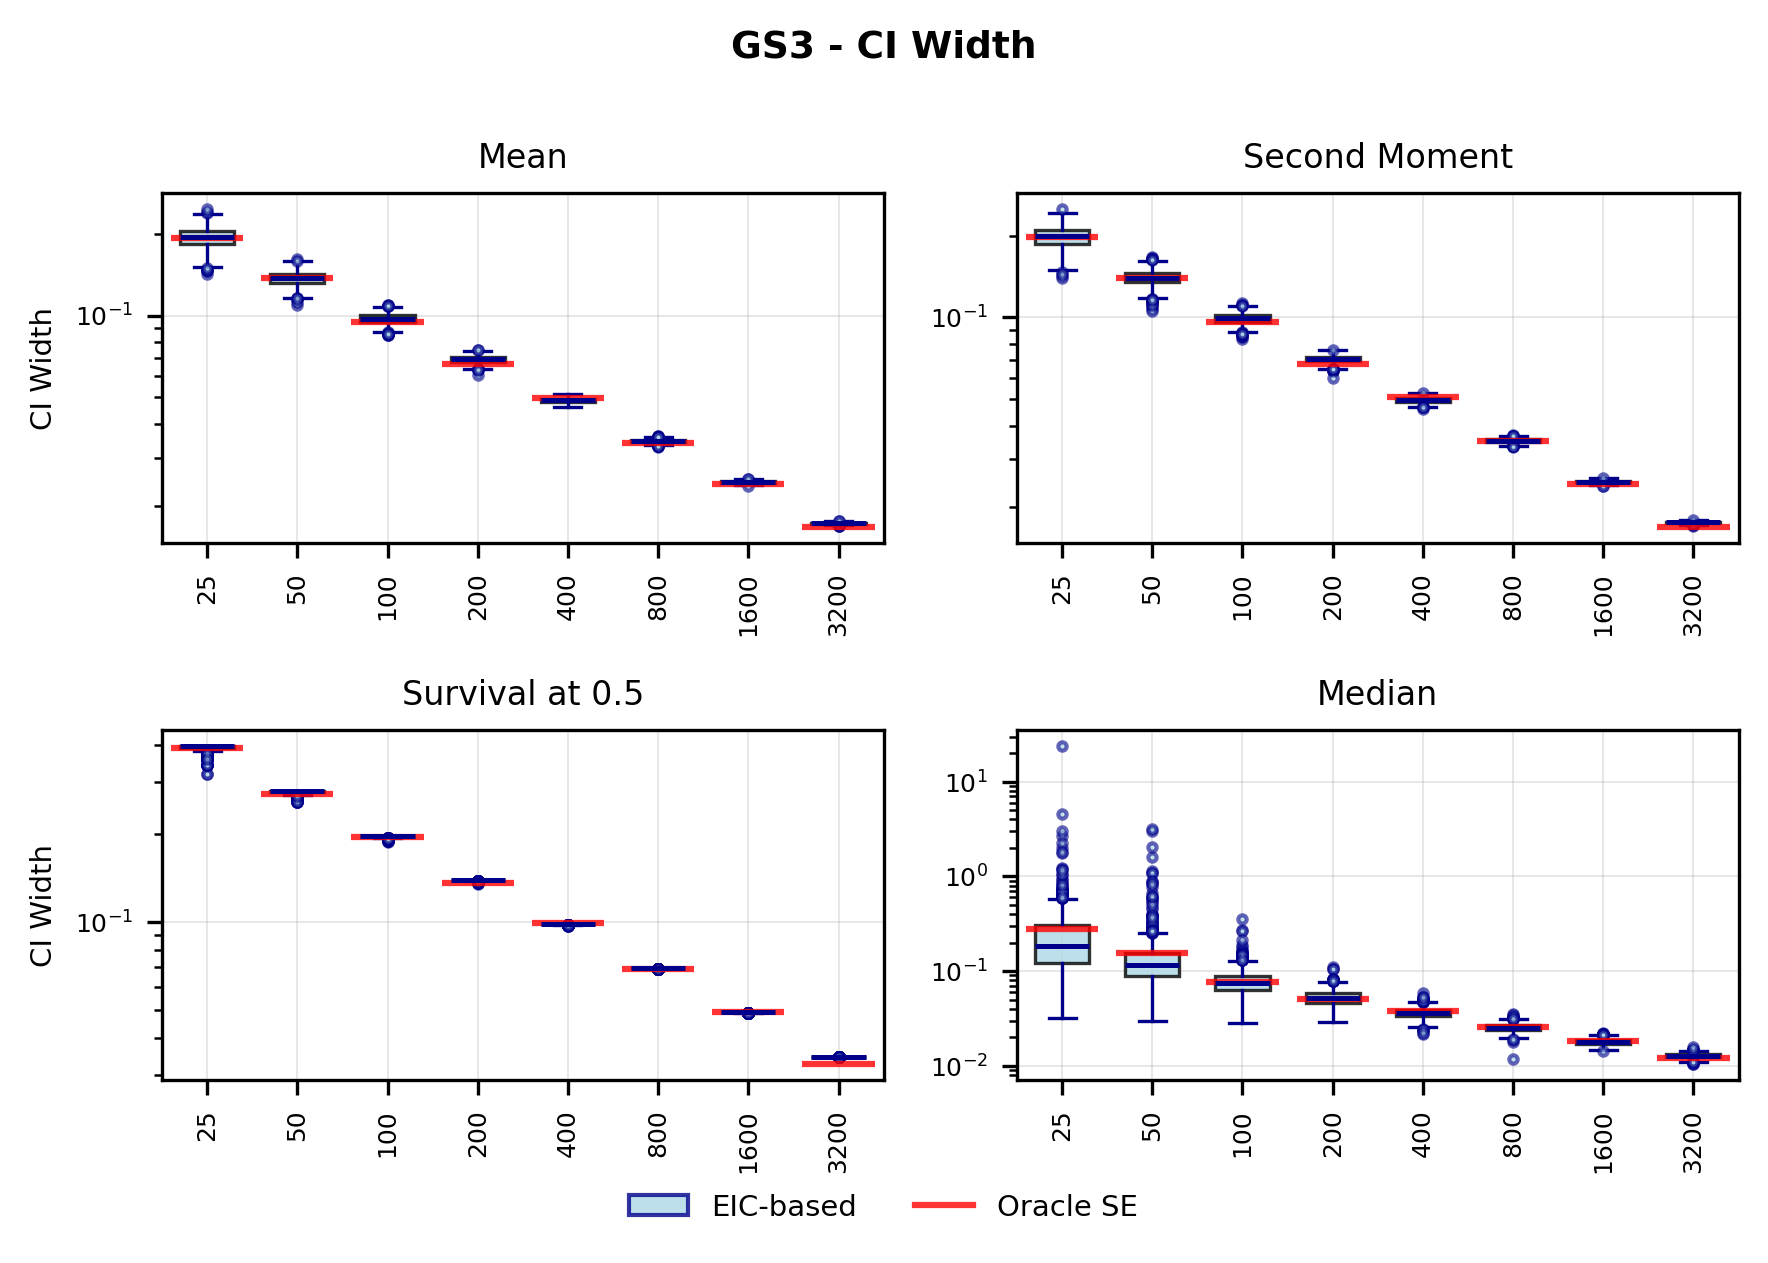
\includegraphics[width=0.75\textwidth]{resources/target_estimand_variance/Figure_CI_Width_TruncatedGMMSymmetricThree.png}
    \caption{EIC\textendash based variance estimation for GS3: CI width.}
\end{figure}

\begin{figure}[H]
    \centering
    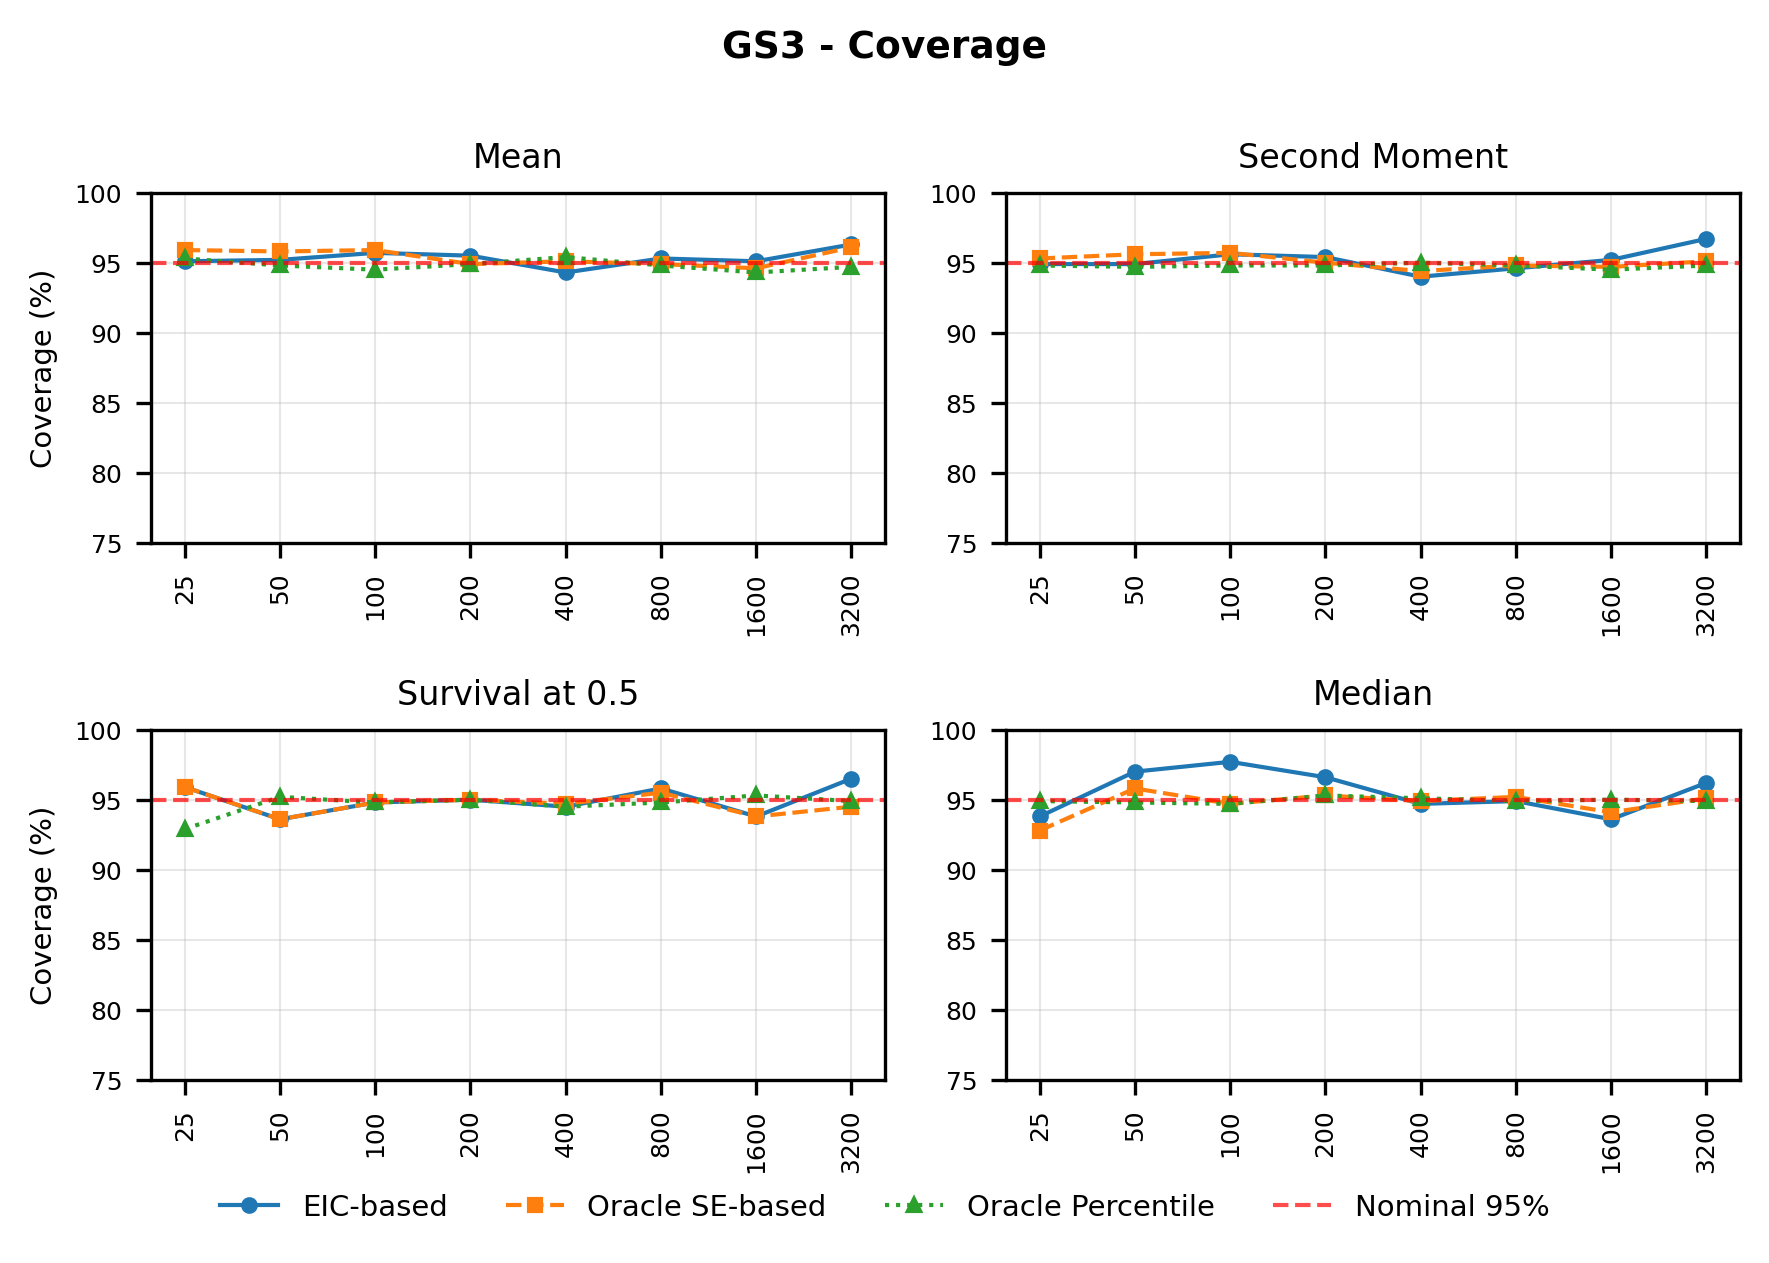
\includegraphics[width=0.75\textwidth]{resources/target_estimand_variance/Figure_Coverage_TruncatedGMMSymmetricThree.png}
    \caption{EIC\textendash based variance estimation for GS3: coverage.}
\end{figure}

\begin{figure}[H]
    \centering
    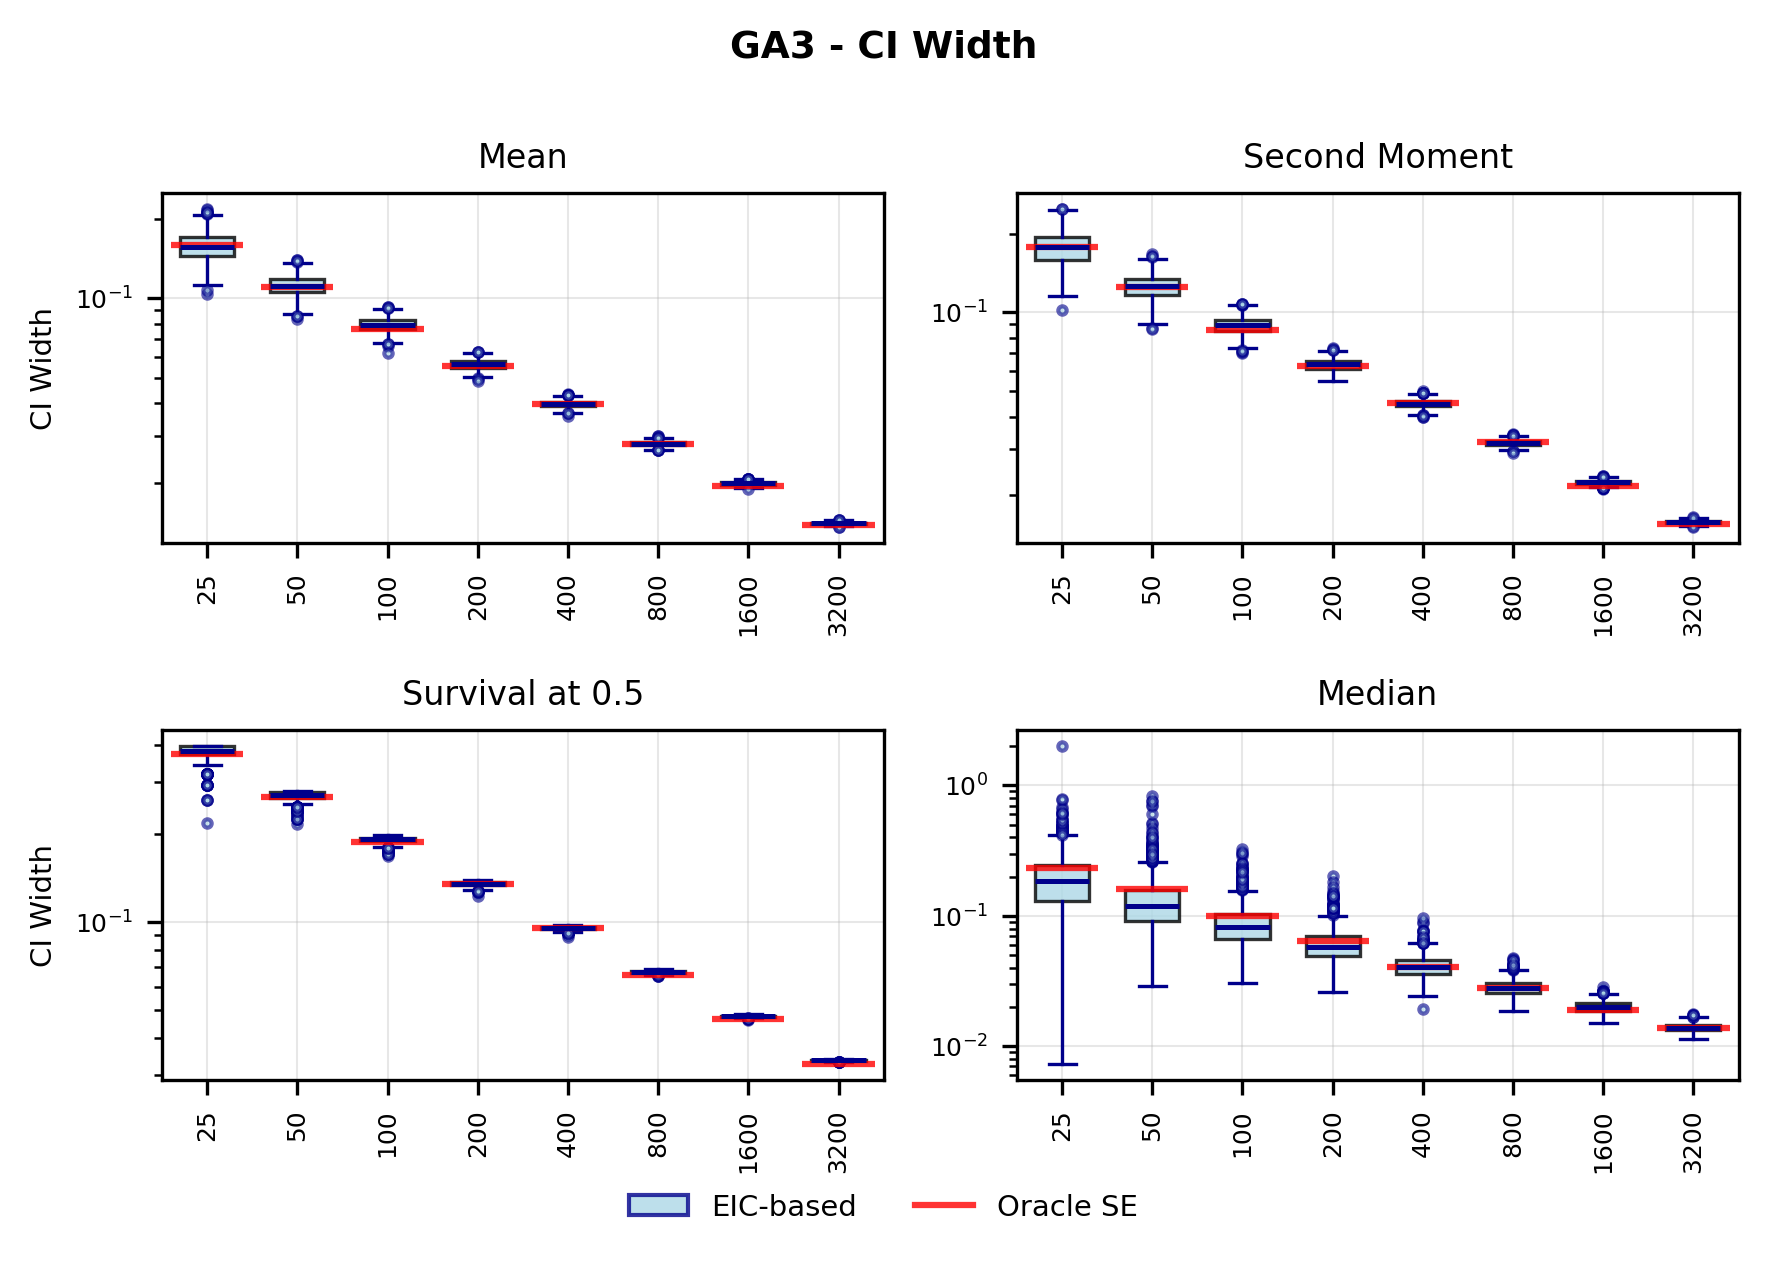
\includegraphics[width=0.75\textwidth]{resources/target_estimand_variance/Figure_CI_Width_TruncatedGMMAsymmetricThree.png}
    \caption{EIC\textendash based variance estimation for GA3: CI width.}
\end{figure}

\begin{figure}[H]
    \centering
    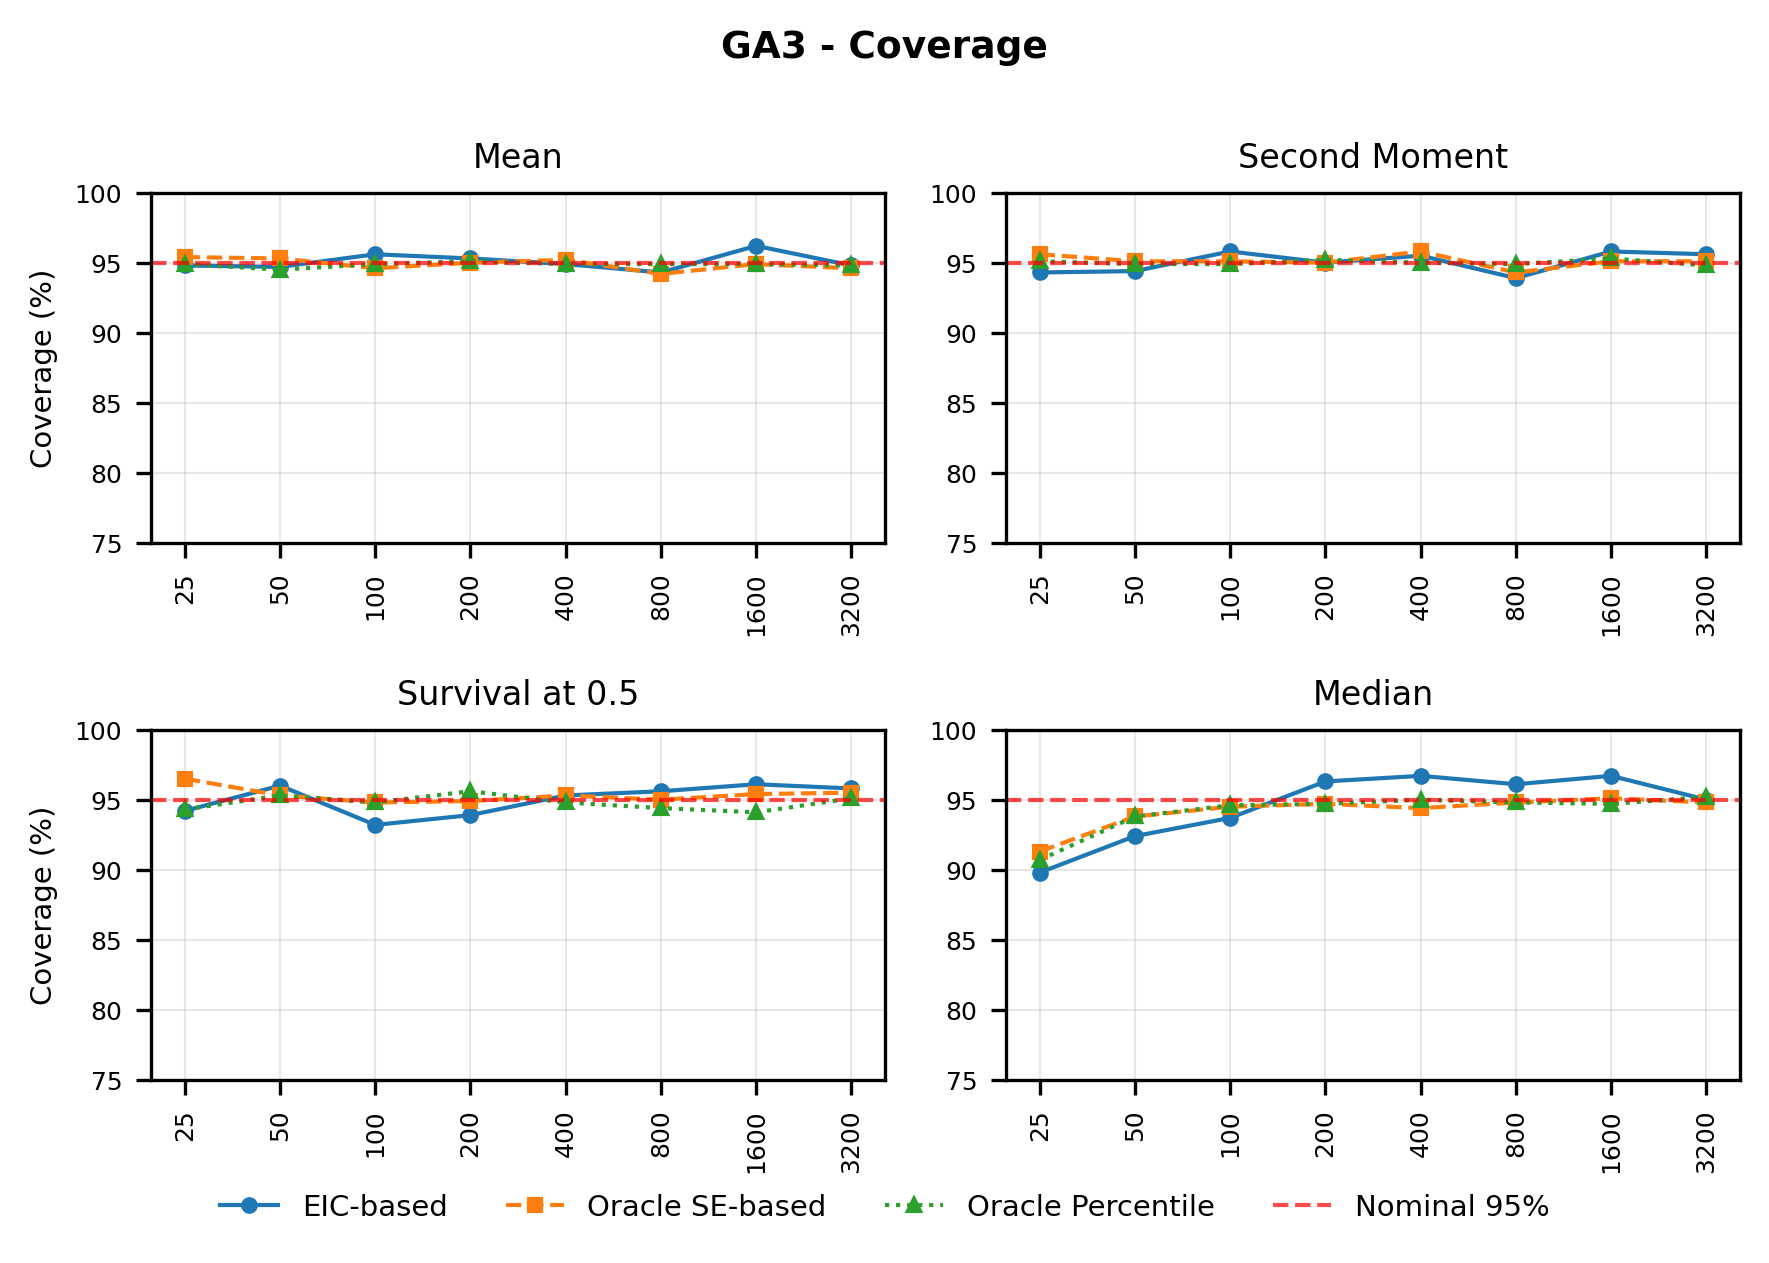
\includegraphics[width=0.75\textwidth]{resources/target_estimand_variance/Figure_Coverage_TruncatedGMMAsymmetricThree.png}
    \caption{EIC\textendash based variance estimation for GA3: coverage.}
\end{figure}

\begin{figure}[H]
    \centering
    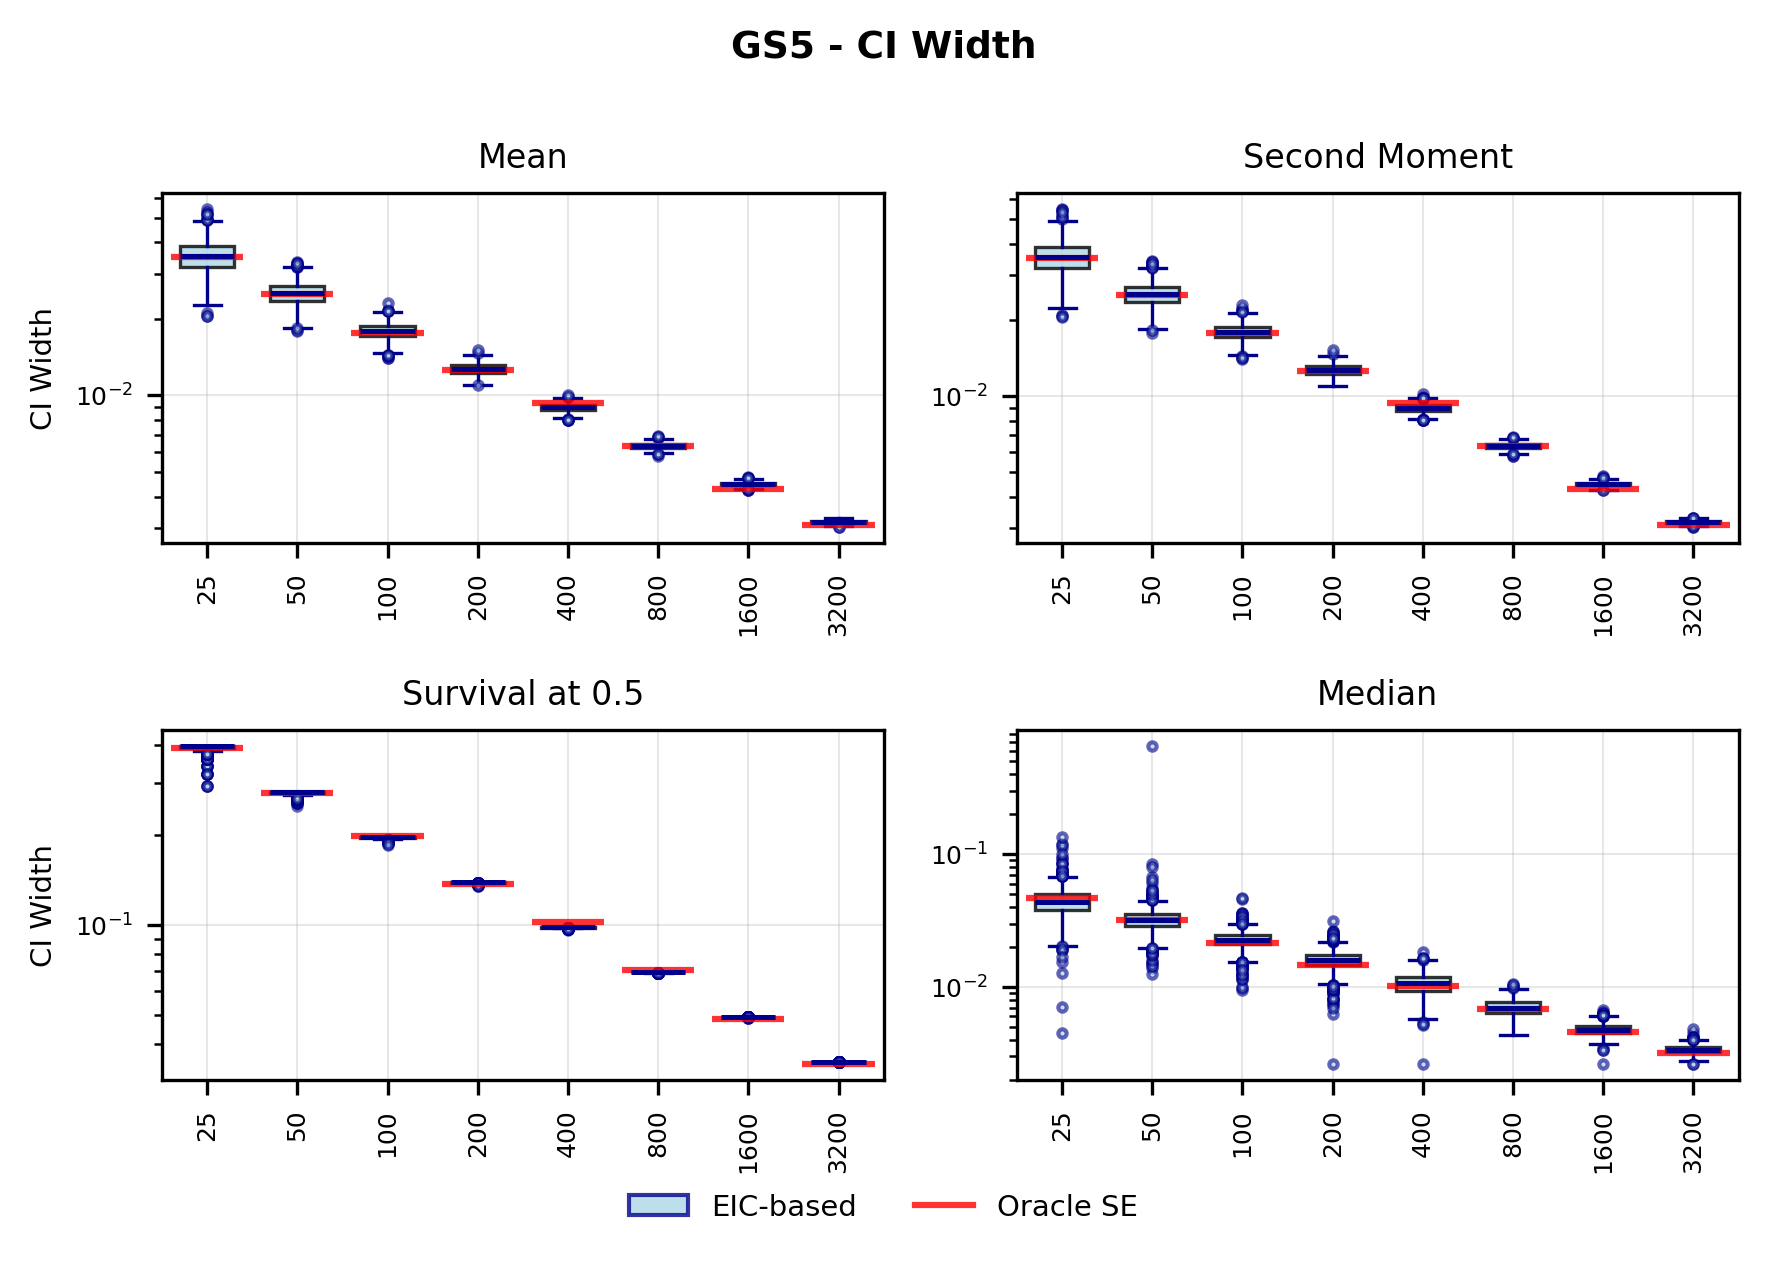
\includegraphics[width=0.75\textwidth]{resources/target_estimand_variance/Figure_CI_Width_TruncatedGMMFiveSpikes.png}
    \caption{EIC\textendash based variance estimation for GS5: CI width.}
\end{figure}

\begin{figure}[H]
    \centering
    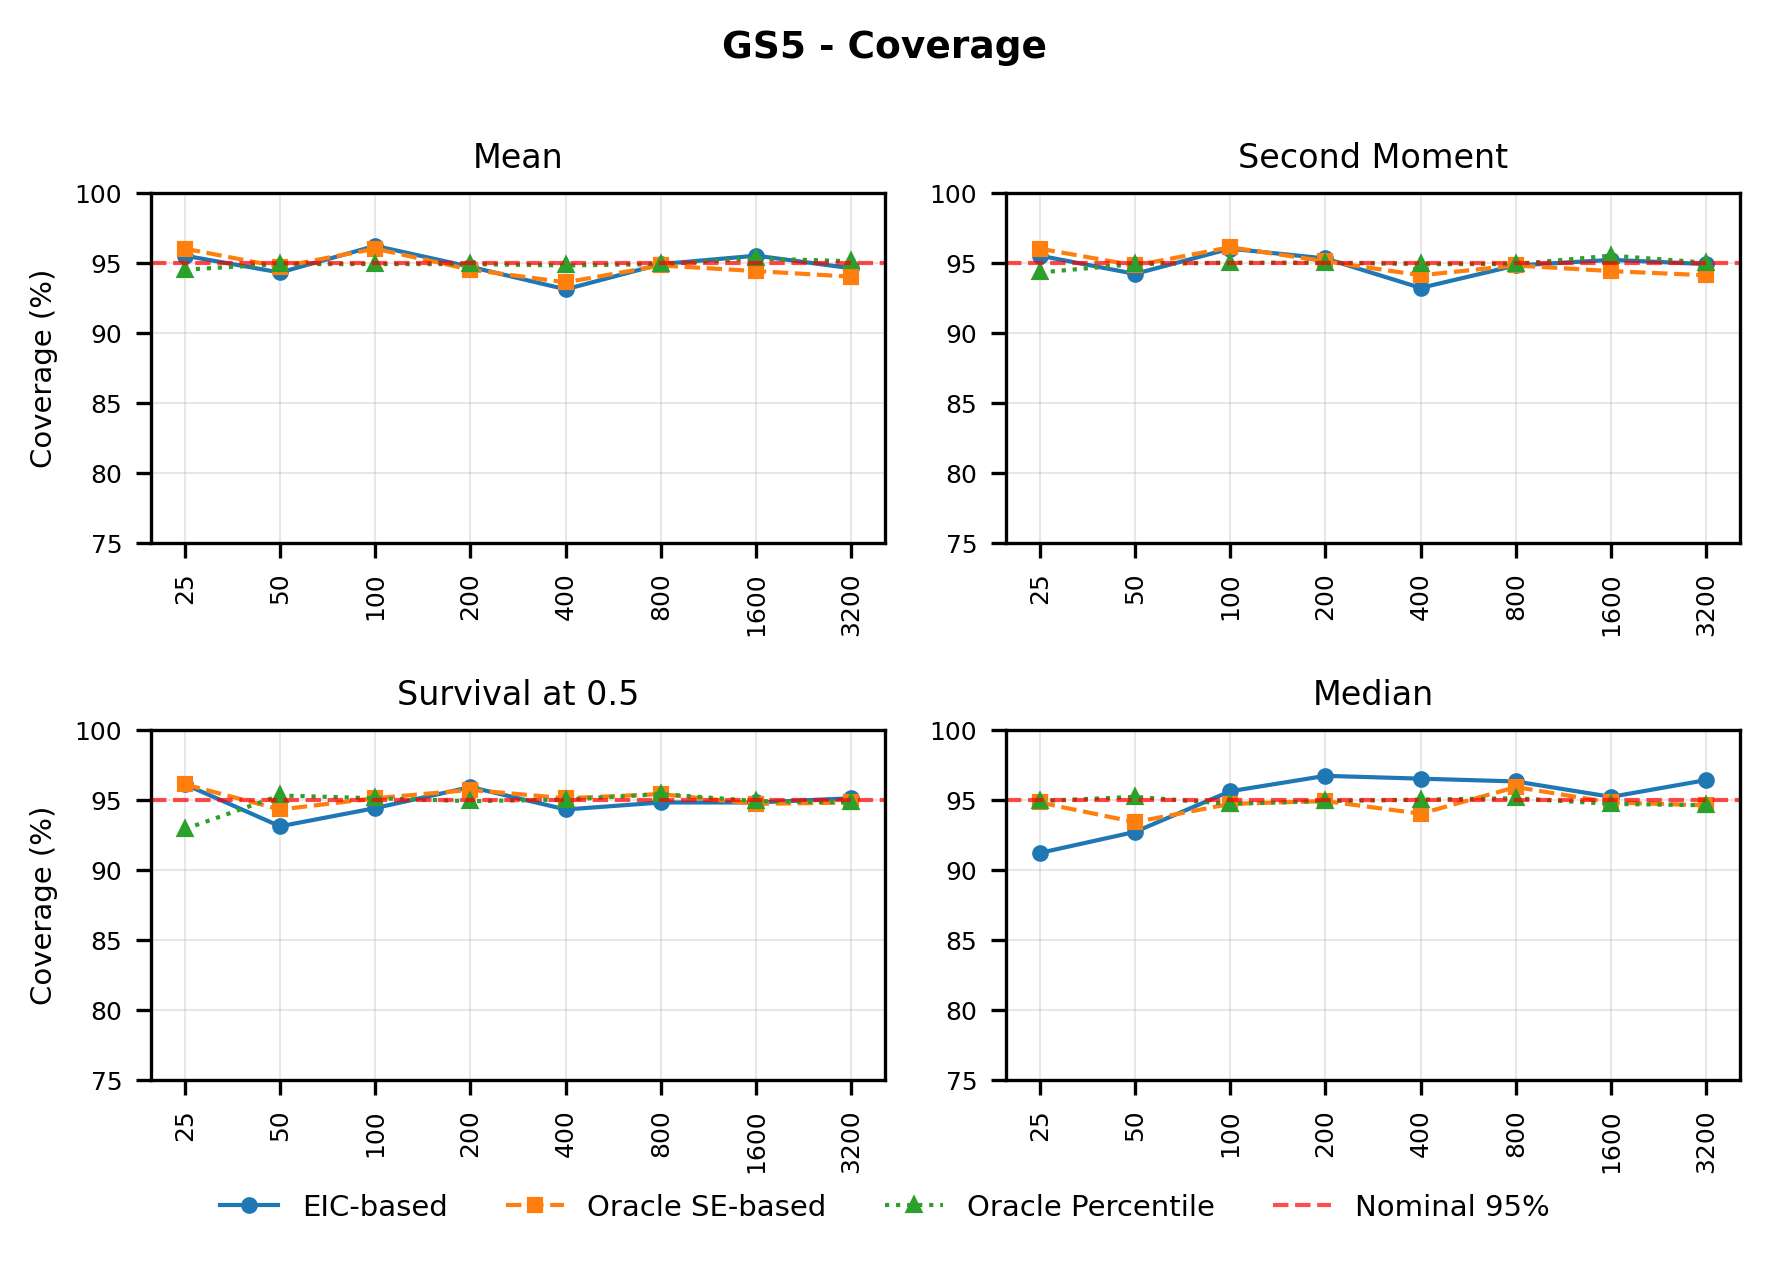
\includegraphics[width=0.75\textwidth]{resources/target_estimand_variance/Figure_Coverage_TruncatedGMMFiveSpikes.png}
    \caption{EIC\textendash based variance estimation for GS5: coverage.}
\end{figure}

\begin{figure}[H]
    \centering
    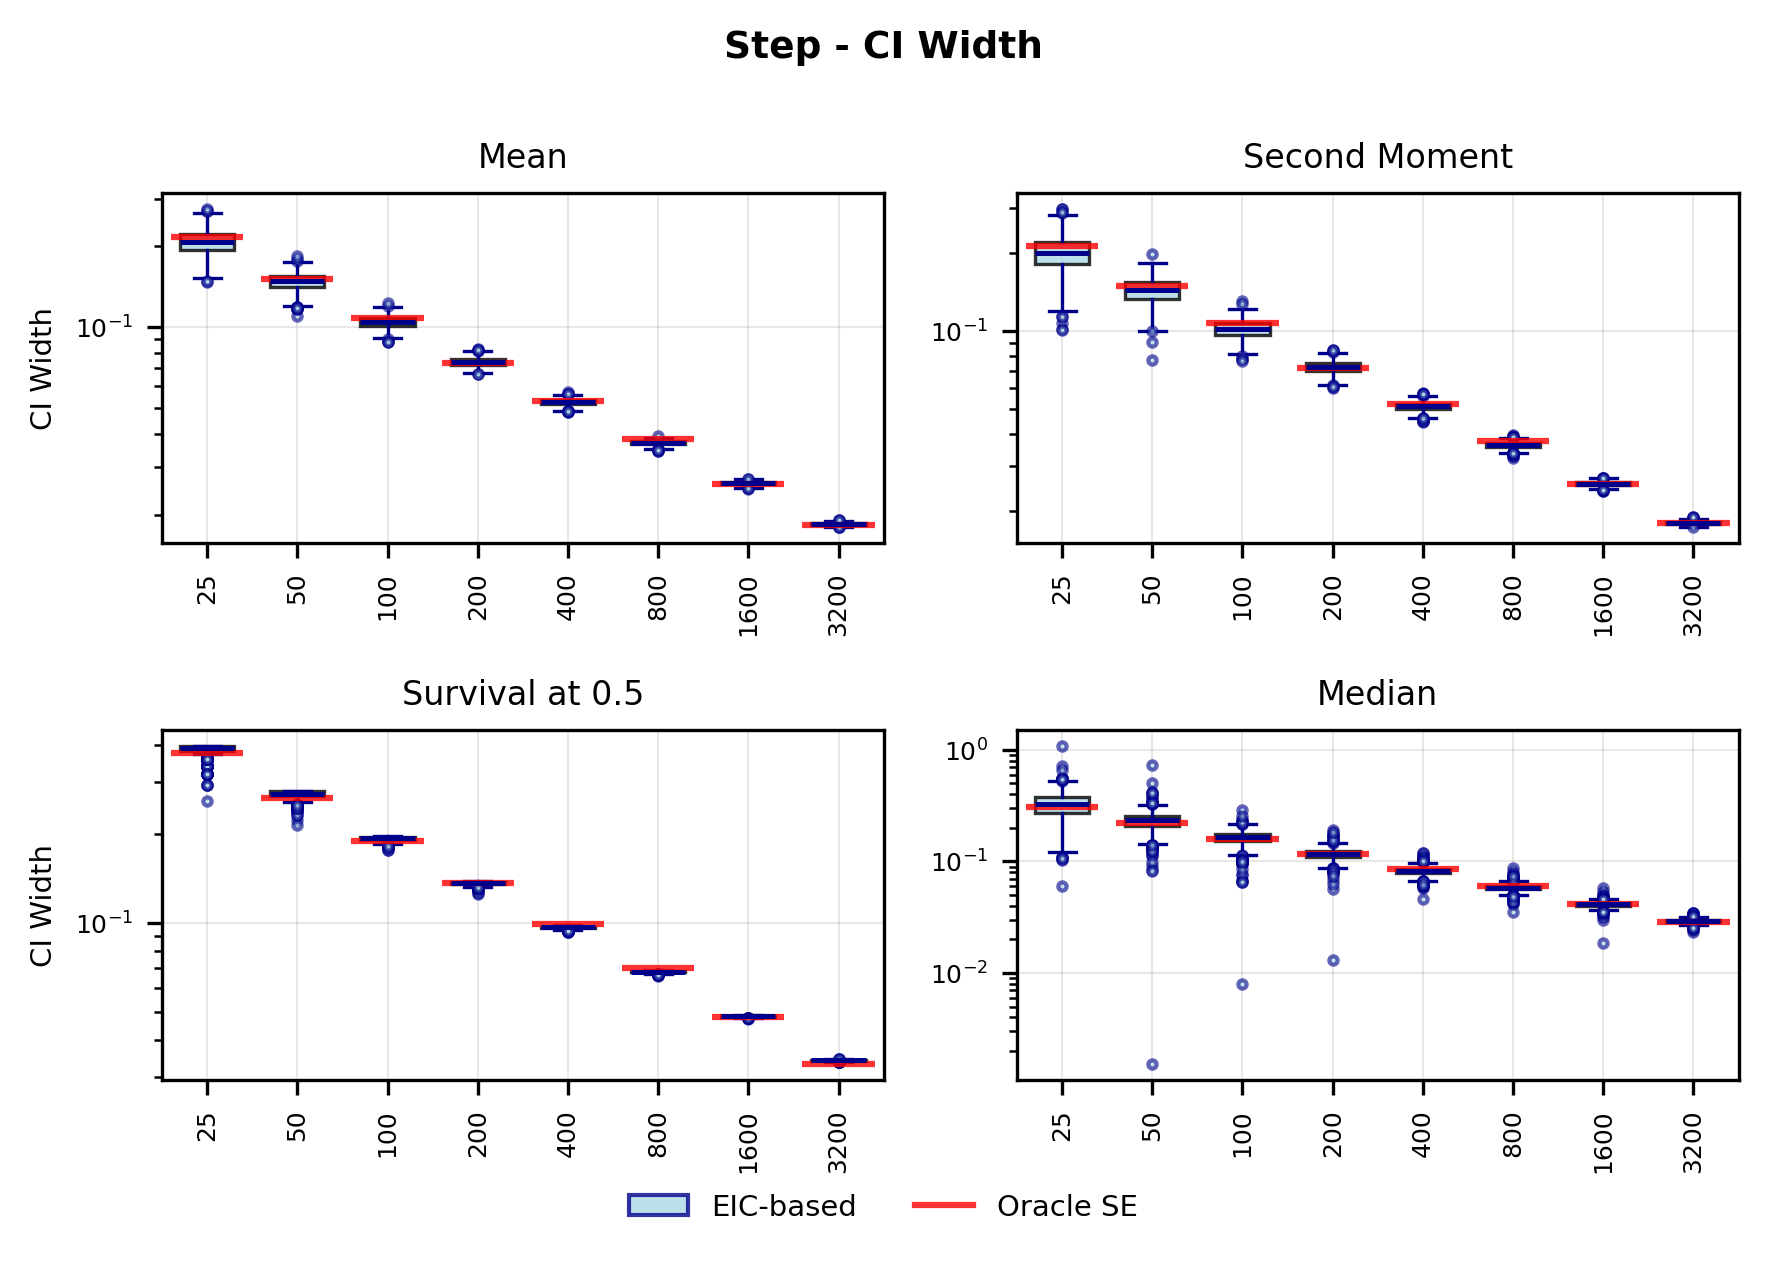
\includegraphics[width=0.75\textwidth]{resources/target_estimand_variance/Figure_CI_Width_StepFunction.png}
    \caption{EIC\textendash based variance estimation for Step: CI width.}
\end{figure}

\begin{figure}[H]
    \centering
    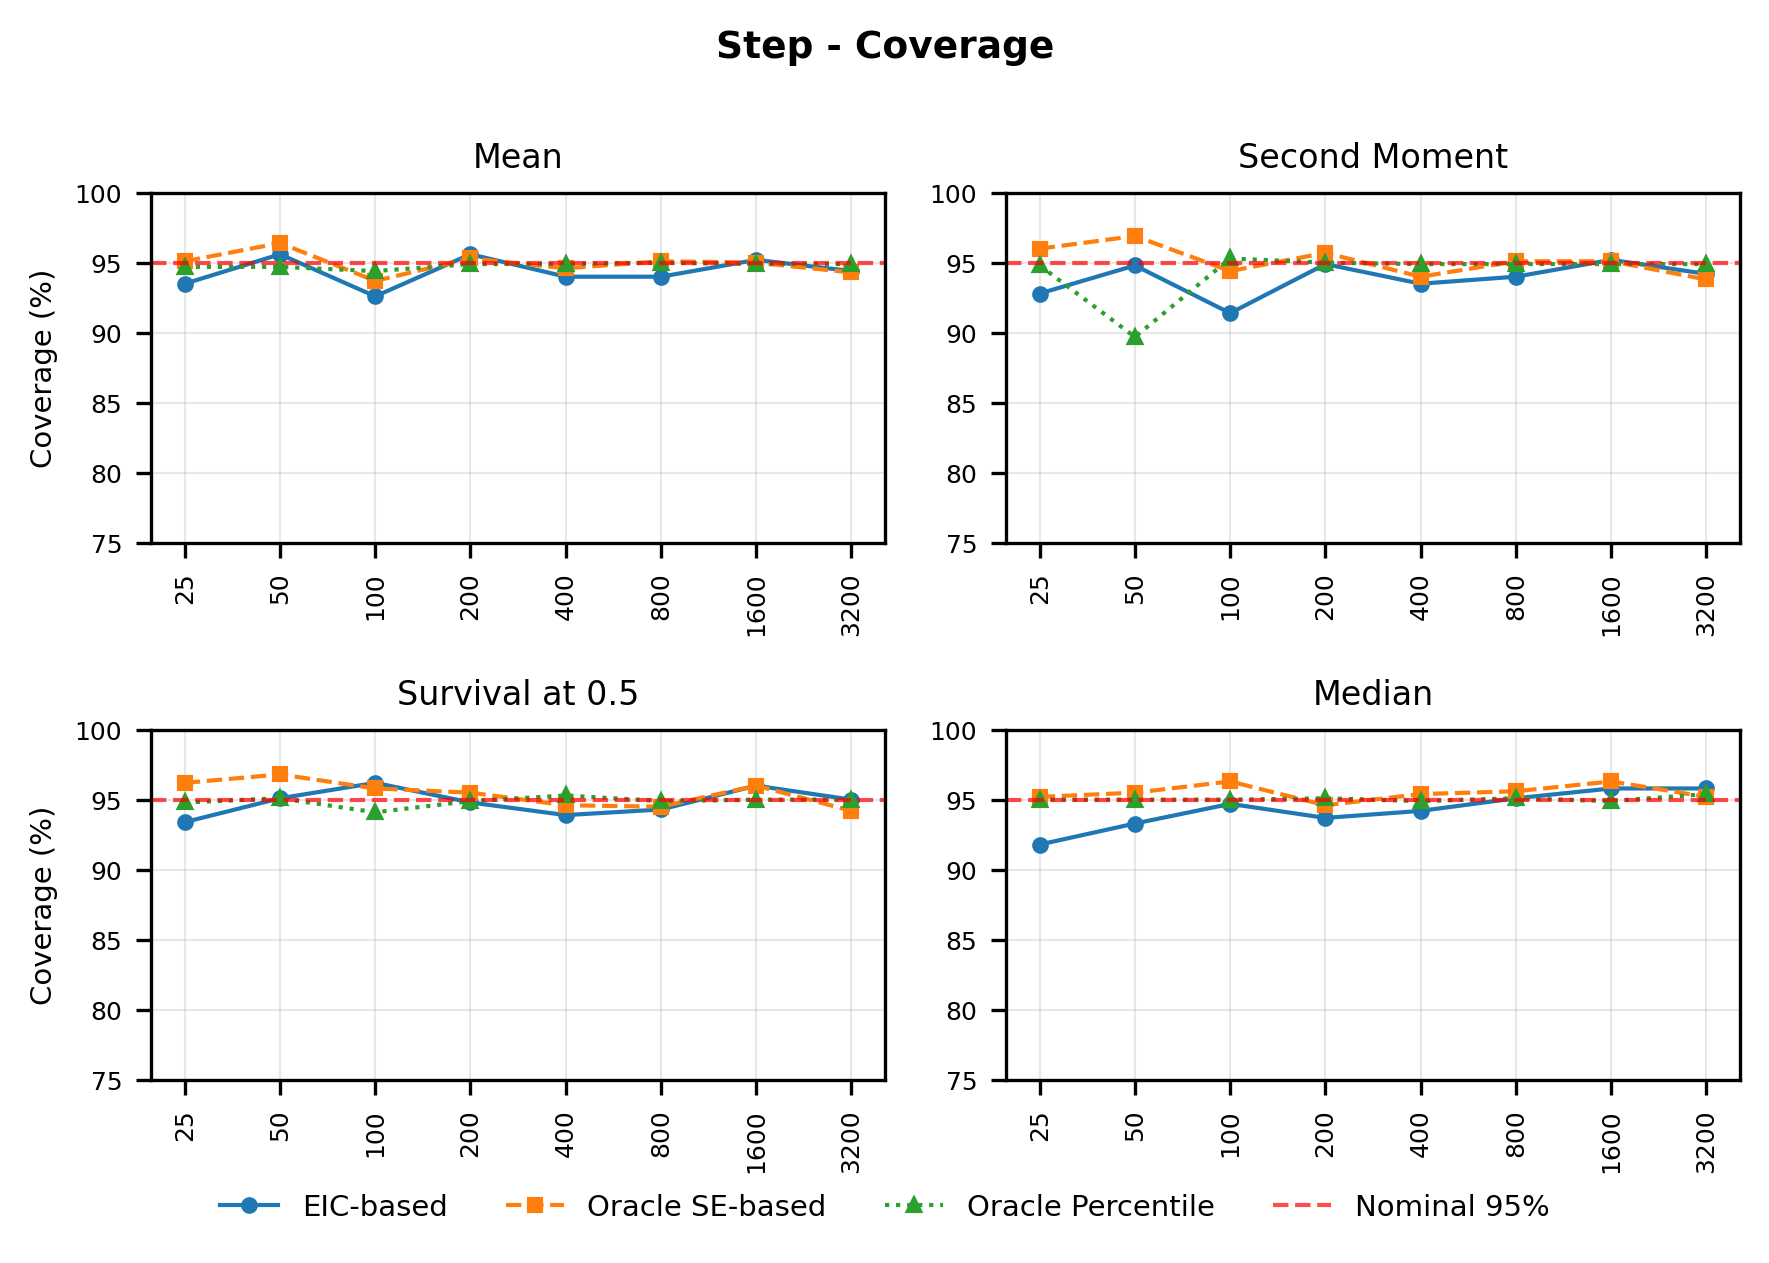
\includegraphics[width=0.75\textwidth]{resources/target_estimand_variance/Figure_Coverage_StepFunction.png}
    \caption{EIC\textendash based variance estimation for Step: coverage.}
\end{figure}

\begin{figure}[H]
    \centering
    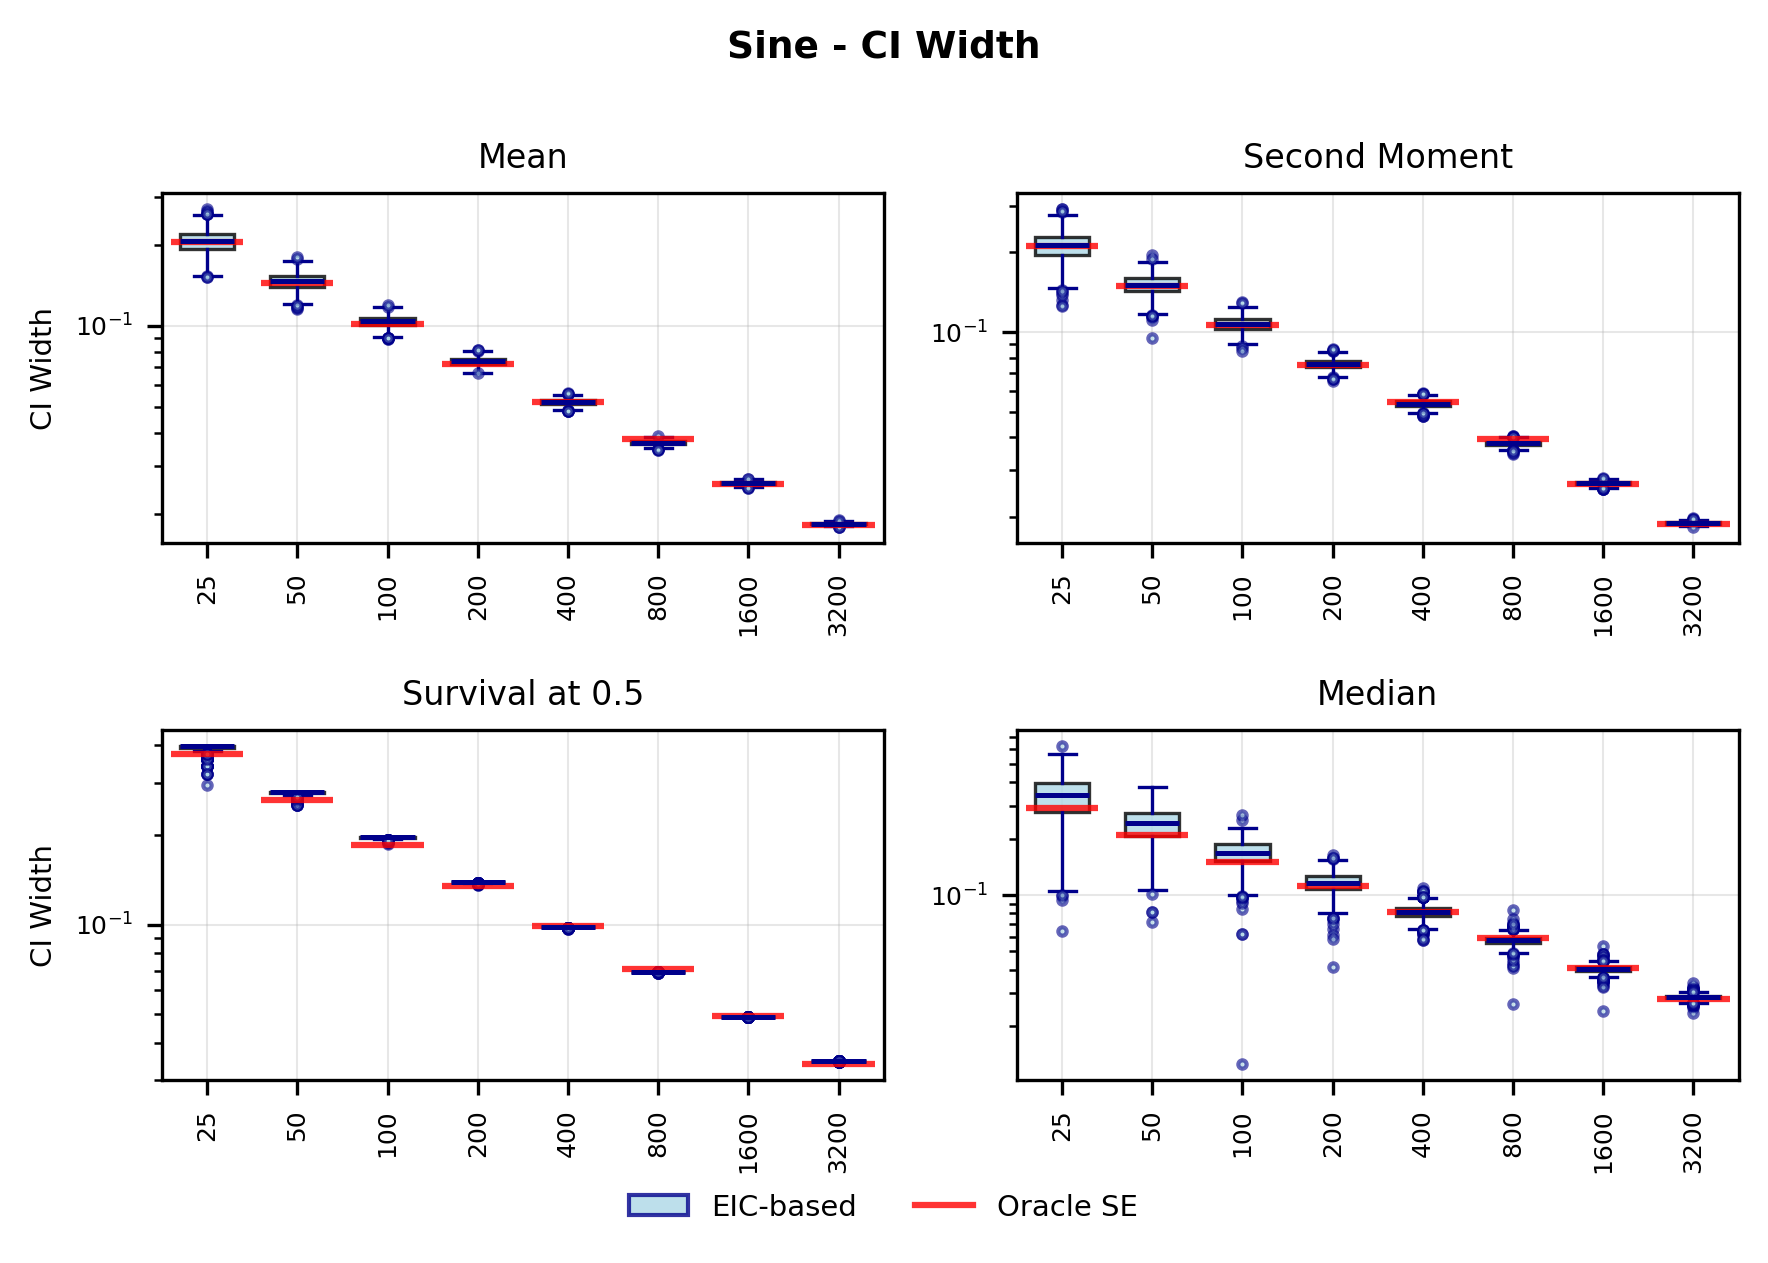
\includegraphics[width=0.75\textwidth]{resources/target_estimand_variance/Figure_CI_Width_Sinusoidal.png}
    \caption{EIC\textendash based variance estimation for Sine: CI width.}
\end{figure}

\begin{figure}[H]
    \centering
    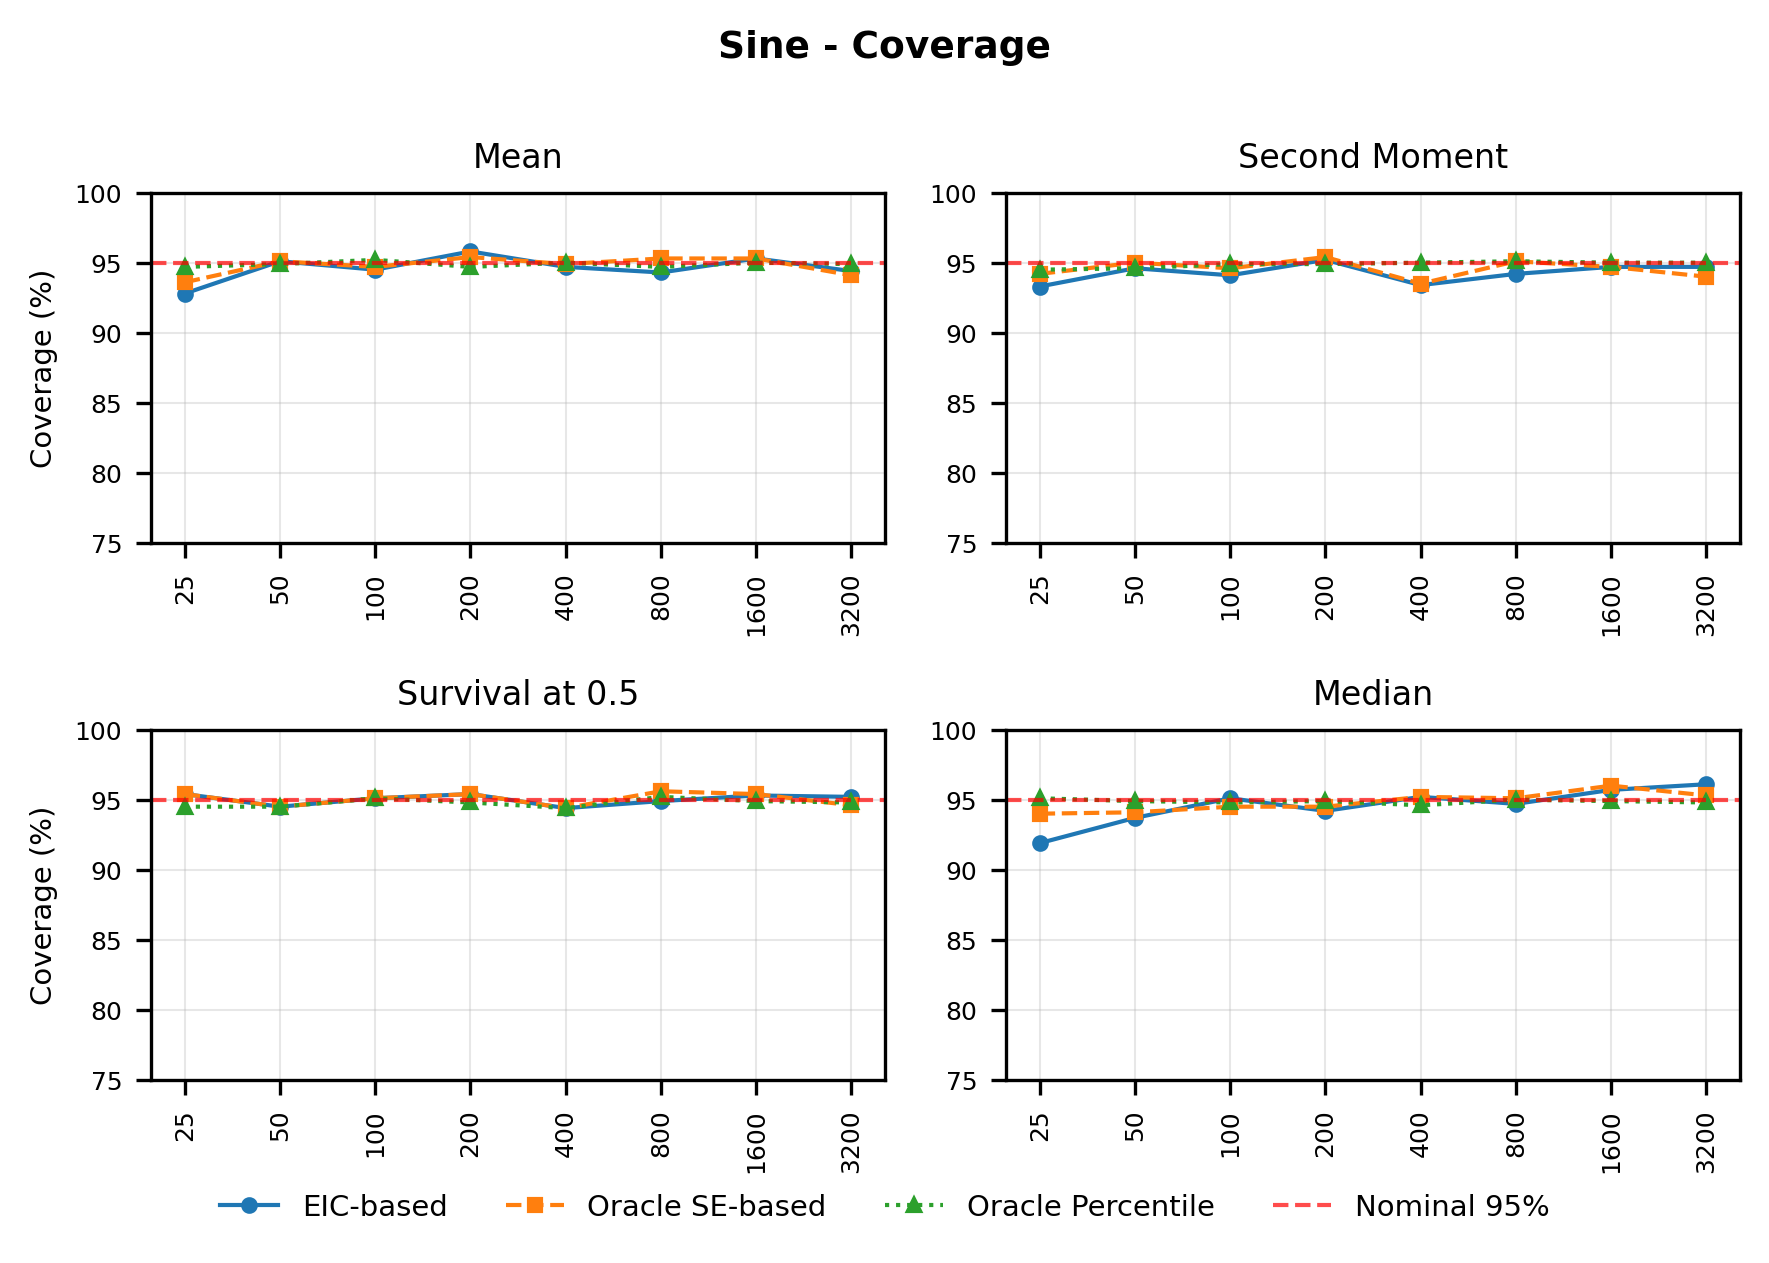
\includegraphics[width=0.75\textwidth]{resources/target_estimand_variance/Figure_Coverage_Sinusoidal.png}
    \caption{EIC\textendash based variance estimation for Sine: coverage.}
\end{figure}

\clearpage
